%% Volume III, Chapter 1: The Real Numbers
\chapter{The Real Numbers}
\label{ch:real-numbers-construction}

\abstract{Volumes~I and~II built the whole of calculus on one assumption, that there is a complete ordered field, and never asked whether such a field exists. It does, and it can be made from the rational numbers alone: a real number is what a sequence of rational approximations, such as the iterates of Heron's method for $\sqrt2$, is trying to reach. Making this precise proves the assumption, shows that the real numbers are determined by it up to a unique isomorphism, and explains why completeness can be stated in so many ways, through suprema, monotone limits, nested intervals, convergent subsequences or Cauchy sequences. The same construction returns in the next chapter, where it completes an arbitrary metric space, and in the spaces of integrable functions of Part~III.}

Every theorem of analysis in Volumes~I and~II goes back to \vcref{1}{asm:reals}: there is a complete ordered field, that is, an ordered field in which every nonempty set that is bounded above has a supremum. The natural numbers were described by Peano's axioms (\vcref{1}{asm:peano}), and the integers and the rational numbers were then \emph{constructed} from them, as classes of pairs (\vcref{1}{sec:integers,sec:rationals}). The real numbers alone were postulated. \Vcref{1}{sec:reals} showed that $\mathbb Q$ is not complete, and the note at its end outlined two ways of filling the gaps; \vcref{1}{thm:r-unique} stated that a complete ordered field is unique, with a sketch of the proof. This chapter carries out the programme in full. \Cref{thm:reals-exist} constructs a complete ordered field from $\mathbb Q$, and \cref{thm:uniqueness-complete} proves that any two complete ordered fields are related by exactly one isomorphism. After that, \vcref{1}{asm:reals} is a theorem, and the whole edifice of Volumes~I and~II rests on the axioms for $\mathbb N$.

A construction of this kind must avoid a trap. Almost every result about limits in Volume~I was proved for real numbers, and many of them use completeness: the monotone convergence theorem, the Bolzano--Weierstrass theorem and the Cauchy criterion all do. Before the construction is finished we must not use any of them, since we are about to prove the assumption on which they rest. Until the end of \cref{sec:completeness-proof} we therefore use from Volume~I only the construction and the properties of $\mathbb N$, $\mathbb Z$ and $\mathbb Q$ (\vcref{1}{sec:naturals,sec:integers,sec:rationals}), equivalence relations and classes (\vcref{1}{ch:sets}), and the results on ordered fields in general: the rules for inequalities, \vcref{1}{prop:order-rules,prop:field-order}, and the properties of the absolute value, \vcref{1}{prop:abs,cor:reverse-triangle}. The last two were stated for real numbers, but, as Volume~I remarked after \vcref{1}{thm:r-unique}, their proofs use only the axioms of an ordered field. Where we need an argument of Volume~I in a general ordered field, we say so and check that it uses nothing else. Once \cref{thm:reals-exist} is proved, the constructed field satisfies \vcref{1}{asm:reals}, and from then on every result of Volumes~I and~II holds for it and is cited freely.

\Cref{sec:ordered-fields} collects what holds in every ordered field: the rational numbers are contained in each of them, sequences, limits and Cauchy sequences make sense in each, and the Archimedean property may or may not hold. \Cref{sec:cauchy-construction} constructs a field $\mathbb R$ from the Cauchy sequences of rational numbers and orders it, and \cref{sec:completeness-proof} proves that it is complete. \Cref{sec:dedekind} describes Dedekind's alternative construction by cuts. \Cref{sec:uniqueness} proves the uniqueness of complete ordered fields, and \cref{sec:forms-completeness} proves the equivalence of the various forms of completeness, which a note of \vcref{1}{ch:limits} stated without proof, with examples showing where the Archimedean property is needed. \Cref{sec:extended-limsup} introduces the extended real line and develops the upper and lower limits, which the later chapters use constantly, \cref{sec:continuum} determines the cardinality of several sets of real numbers and of functions, with the Cantor set and Liouville's transcendental numbers, and \cref{sec:real-computation} looks at real numbers as rational sequences and at the floating-point numbers that stand in for them on a computer.

Throughout the chapter, $F$ denotes an ordered field with the set $P$ of positive elements (\vcref{1}{def:ordered}), and $x<y$ means $y-x\in P$. When we speak of a tolerance $\varepsilon>0$ in $F$, we mean an element of $P$, not only a rational one; whether this makes a difference is one of the themes of the chapter. In $\mathbb Q$, tolerances are positive rational numbers. Sequences are indexed by $n\in\mathbb N$, starting from $0$, unless stated otherwise.

\section{Ordered Fields}
\label{sec:ordered-fields}

An ordered field is a set with addition, multiplication and a set of positive elements that satisfy the axioms of \vcref{1}{tab:axioms}: the eight axioms of a commutative ring, the existence of inverses (M4), $0\ne1$ (N), trichotomy (O1) and the closure of the positive elements under sums and products (O2). The rational numbers form an ordered field (\vcref{1}{thm:q-ordered}), and so do the real numbers of Volume~I. Not every field can be ordered. In an ordered field $1>0$, so the sums $1$, $1+1$, $1+1+1$, \ldots\ are all positive and hence nonzero; the field $\mathbb Z/p\mathbb Z$ of \vcref{1}{cor:zp-field}, in which $p$ ones add up to $0$, therefore has no order, and neither does $\mathbb C$, in which $i^2=-1$ would have to be positive (\vcref{1}{prop:c-not-ordered}). This section collects what every ordered field has, beginning with a copy of $\mathbb Q$.

\subsection{The Rational Elements}

The elements $0$, $1$, $1+1$, \ldots\ of an ordered field behave like the natural numbers, their negatives like the integers, and their quotients like the rational numbers. Volume~I observed this informally after \vcref{1}{asm:reals}; here is the precise statement. For $n\in\mathbb N$ we write $n\cdot1$ for the element of $F$ defined recursively by $0\cdot1\coloneqq0$ and $(n+1)\cdot1\coloneqq n\cdot1+1$, which is legitimate by the recursion theorem, \vcref{1}{thm:recursion}.

\begin{proposition}[The rational elements of an ordered field]
\label{prop:prime-field}
Let $F$ be an ordered field. There is exactly one map $\iota\colon\mathbb Q\to F$ with
\[
\iota(1)=1,\qquad\iota(a+b)=\iota(a)+\iota(b),\qquad\iota(ab)=\iota(a)\,\iota(b)\qquad(a,b\in\mathbb Q).
\]
It satisfies $\iota(n)=n\cdot1$ for $n\in\mathbb N$, and it is strictly increasing: $a<b$ implies $\iota(a)<\iota(b)$. In particular $\iota$ is injective.
\end{proposition}

\begin{proof}
\emph{Existence on $\mathbb N$.} Put $e(n)\coloneqq n\cdot1$. By induction on $n$, $e(m+n)=e(m)+e(n)$: for $n=0$ both sides are $e(m)$, and $e(m+n+1)=e(m+n)+1=e(m)+e(n)+1=e(m)+e(n+1)$. Then $e(mn)=e(m)\,e(n)$, again by induction on $n$, since $e(m(n+1))=e(mn+m)=e(m)e(n)+e(m)=e(m)\bigl(e(n)+1\bigr)$ by the distributive law. Moreover $e(n)>0$ for $n\ge1$, because $e(1)=1>0$ and $e(n+1)=e(n)+1$ is a sum of positive elements. Consequently $m<n$ implies $e(n)=e(m)+e(n-m)>e(m)$.

\emph{Existence on $\mathbb Z$.} By \vcref{1}{def:integers}, an integer is a class $[(a,b)]$ of pairs of natural numbers, with $(a,b)\sim(c,d)$ if and only if $a+d=b+c$. Put $e([(a,b)])\coloneqq e(a)-e(b)$. This is well defined: $a+d=b+c$ gives $e(a)+e(d)=e(b)+e(c)$, that is, $e(a)-e(b)=e(c)-e(d)$. Sums of classes are formed componentwise, so $e$ is additive, and the product $[(a,b)]\,[(c,d)]=[(ac+bd,\,ad+bc)]$ is mapped to $e(a)e(c)+e(b)e(d)-e(a)e(d)-e(b)e(c)=\bigl(e(a)-e(b)\bigr)\bigl(e(c)-e(d)\bigr)$. On $\mathbb N$, which is embedded in $\mathbb Z$ by $n\mapsto[(n,0)]$, the new $e$ agrees with the old one. An integer $m>0$ is a natural number $n\ge1$ (\vcref{1}{prop:z-sign}), and $e(m)=n\cdot1>0$; hence $e(m)<0$ for $m<0$, and $e(m)\ne0$ for $m\ne0$.

\emph{Existence on $\mathbb Q$.} For $p/q\in\mathbb Q$ put $\iota(p/q)\coloneqq e(p)\,e(q)^{-1}$. If $p/q=r/s$, then $ps=qr$, so $e(p)e(s)=e(q)e(r)$, and multiplying by $e(q)^{-1}e(s)^{-1}$ gives $e(p)e(q)^{-1}=e(r)e(s)^{-1}$; so $\iota$ is well defined. Since $p/q+r/s=(ps+qr)/(qs)$,
\[
\iota\Bigl(\frac pq+\frac rs\Bigr)=\frac{e(p)e(s)+e(q)e(r)}{e(q)e(s)}=\frac{e(p)}{e(q)}+\frac{e(r)}{e(s)},
\]
and products are treated in the same way. On $\mathbb Z$, $\iota(p/1)=e(p)$, and $\iota(1)=1$. Finally, a rational number $x>0$ can be written $x=p/q$ with $q>0$, and then $p>0$, by \vcref{1}{thm:q-ordered}; so $e(p)>0$ and $e(q)>0$, and $\iota(x)=e(p)\,e(q)^{-1}>0$ by \vcref{1}{prop:field-order}\,(i). If $a<b$, then $\iota(b)-\iota(a)=\iota(b-a)>0$.

\emph{Uniqueness.} Let $\kappa\colon\mathbb Q\to F$ be any map with the three properties. From $\kappa(0)=\kappa(0+0)=\kappa(0)+\kappa(0)$ we get $\kappa(0)=0$, and $\kappa(n+1)=\kappa(n)+\kappa(1)=\kappa(n)+1$, so $\kappa(n)=n\cdot1=e(n)$ for all $n\in\mathbb N$ by induction. For an integer $m$, $\kappa(m)+\kappa(-m)=\kappa(0)=0$, so $\kappa(-m)=-\kappa(m)$, and $\kappa=e$ on $\mathbb Z$. For a fraction $p/q$ we have $\kappa(q)\,\kappa(p/q)=\kappa(p)$, that is, $e(q)\,\kappa(p/q)=e(p)$, and since $e(q)\ne0$, $\kappa(p/q)=e(p)\,e(q)^{-1}=\iota(p/q)$.
\end{proof}

The image $\iota(\mathbb Q)$ is a copy of $\mathbb Q$ inside $F$, with the same sums, products and order, and we shall identify each rational number $q$ with the element $\iota(q)$, calling these elements the \term{rational elements} of $F$. In this sense $\mathbb N\subset\mathbb Z\subset\mathbb Q\subseteq F$ for every ordered field $F$, and in particular every ordered field is infinite. The proposition also shows that the copy is unique: there is no second way of placing $\mathbb Q$ inside $F$ that respects the arithmetic. In the language of algebra, $\mathbb Q$ is the \term{prime field} of every ordered field. When two ordered fields $F$ and $F'$ are compared, as in \cref{sec:uniqueness}, we write $q$ for the rational element of $F$ and $q'$ for the corresponding element of $F'$.

\subsection{Absolute Value and Sequences}

In an ordered field the \term{absolute value} is defined as in $\mathbb R$: $|x|\coloneqq x$ if $x\ge0$ and $|x|\coloneqq-x$ if $x<0$. Its properties, \vcref{1}{prop:abs,cor:reverse-triangle}, hold in every ordered field with the same proofs: $|x|\ge0$, $|xy|=|x|\,|y|$, $|x|\le c$ if and only if $-c\le x\le c$, the triangle inequality $|x+y|\le|x|+|y|$, and $\bigl||x|-|y|\bigr|\le|x-y|$. With the absolute value we can speak of the distance $|x-y|$ between two elements, and therefore of limits.

\begin{definition}[Convergence in an ordered field]
\label{def:of-convergence}
Let $F$ be an ordered field and $(a_n)$ a sequence in $F$.
\begin{enumerate}
\item $(a_n)$ \term{converges} to $L\in F$, written $a_n\to L$, if for every $\varepsilon>0$ in $F$ there is $N\in\mathbb N$ with $|a_n-L|<\varepsilon$ for all $n\ge N$. A sequence that converges to $0$ is a \term{null sequence}.
\item $(a_n)$ is a \term{Cauchy sequence} if for every $\varepsilon>0$ in $F$ there is $N\in\mathbb N$ with $|a_m-a_n|<\varepsilon$ for all $m,n\ge N$.
\item $(a_n)$ is \term{bounded} if there is $C\in F$ with $|a_n|\le C$ for all $n$; it is \term{bounded above} if there is $C$ with $a_n\le C$ for all $n$, and \term{bounded below} similarly. It is \term{increasing} if $a_n\le a_{n+1}$ for all $n$, and \term{decreasing} if $a_n\ge a_{n+1}$ for all $n$.
\end{enumerate}
\end{definition}

For $F=\mathbb R$ these are the definitions of \vcref{1}{def:sequence-limit,def:cauchy}, and for $F=\mathbb Q$ they are those of the note at the end of \vcref{1}{sec:reals}, with rational tolerances. The tolerance $\varepsilon$ ranges over all positive elements of $F$. In $\mathbb Q$ and $\mathbb R$ it would make no difference to use only the tolerances $1/k$, $k\ge1$, but we shall soon meet a field in which it does. The basic rules for limits hold in every ordered field.

\begin{proposition}[Limits in an ordered field]
\label{prop:of-limits}
Let $F$ be an ordered field, and let $(a_n)$ and $(b_n)$ be sequences in $F$.
\begin{enumerate}
\item A sequence has at most one limit.
\item Every convergent sequence is a Cauchy sequence, and every Cauchy sequence is bounded.
\item If $a_n\to L$ and $b_n\to M$, then $a_n+b_n\to L+M$, $a_n-b_n\to L-M$ and $a_nb_n\to LM$; if moreover $M\ne0$, then $b_n\ne0$ for all sufficiently large $n$, and $a_n/b_n\to L/M$.
\item Let $a_n\to L$ and $b_n\to M$. If $L<M$, then $a_n<b_n$ for all sufficiently large $n$; if $a_n\le b_n$ for all sufficiently large $n$, then $L\le M$. If $a_n\le c_n\le b_n$ for all sufficiently large $n$ and $a_n\to L$, $b_n\to L$, then $c_n\to L$.
\item If $a_n\to L$, then every subsequence of $(a_n)$ converges to $L$.
\item If $(a_n)$ is a Cauchy sequence and a subsequence of $(a_n)$ converges to $L$, then $a_n\to L$.
\end{enumerate}
\end{proposition}

\begin{proof}
The proofs of \vcref{1}{thm:limit-unique,prop:convergent-bounded,thm:limit-laws,prop:limit-order,thm:squeeze,prop:subsequence} apply in $F$ word for word. They use the axioms of an ordered field, the triangle inequality, and tolerances obtained from a given $\varepsilon>0$ by field operations, such as $\varepsilon/2$, $\varepsilon/(2C)$, $\varepsilon/(2|M|+1)$, $|M|^2\varepsilon/2$ and $|L-M|/2$, which are positive elements of $F$; none of them uses the Archimedean property or completeness. This gives (i), (iii), (iv), (v), and the fact that convergent sequences are bounded. The first paragraph of the proof of \vcref{1}{thm:cauchy-criterion} shows that a convergent sequence is a Cauchy sequence, with the same reservation.

For the boundedness of a Cauchy sequence, choose $N$ with $|a_m-a_n|<1$ for $m,n\ge N$. Then $|a_n|\le|a_N|+|a_n-a_N|<|a_N|+1$ for $n\ge N$, and $C\coloneqq\max(|a_0|,\ldots,|a_{N-1}|,|a_N|+1)$ bounds every term. For (vi), let $a_{n_k}\to L$ and $\varepsilon>0$. Choose $N$ with $|a_m-a_n|<\varepsilon/2$ for $m,n\ge N$, and then $k$ with $n_k\ge N$ and $|a_{n_k}-L|<\varepsilon/2$, which is possible because $n_k\ge k$. For $n\ge N$, $|a_n-L|\le|a_n-a_{n_k}|+|a_{n_k}-L|<\varepsilon$.
\end{proof}

What fails in a general ordered field is the converse direction of the Cauchy criterion, that every Cauchy sequence converges, together with everything that rests on completeness. $\mathbb Q$ is the standard example. The Heron iterates $1$, $3/2$, $17/12$, $577/408$, \ldots\ of \vcref{1}{tab:heron} form a Cauchy sequence in $\mathbb Q$, as \cref{sec:cauchy-construction} verifies with rational arithmetic alone, and they have no limit in $\mathbb Q$: a rational limit $L$ would satisfy $L\ge1$ by (iv), since all iterates are at least $1$, and $L=(L+2/L)/2$ by (iii), that is, $L^2=2$, which is impossible by \vcref{1}{thm:sqrt2}.

\subsection{The Archimedean Property}

The second property that separates the ordered fields is the one that Volume~I derived from completeness in \vcref{1}{thm:archimedes}.

\begin{definition}[Archimedean field]
\label{def:archimedean}
An ordered field $F$ is \term{Archimedean} if the set $\mathbb N$ of its natural numbers is not bounded above in $F$: for every $x\in F$ there is $n\in\mathbb N$ with $n>x$.
\end{definition}

The rational numbers are Archimedean, as Volume~I observed after \vcref{1}{prop:field-order}: if $x=p/q$ with $q>0$, then $x\le|p|<|p|+1$. The property has several equivalent forms, which show what it means for limits.

\begin{proposition}[Forms of the Archimedean property]
\label{prop:archimedean-forms}
For an ordered field $F$ the following statements are equivalent.
\begin{enumerate}
\item $F$ is Archimedean.
\item For all $x>0$ and $y$ in $F$ there is $n\in\mathbb N$ with $nx>y$.
\item $1/n\to0$ in $F$, as $n\to\infty$ through the integers $n\ge1$.
\item The rational elements are \term{dense} in $F$: for all $x<y$ in $F$ there is a rational $q$ with $x<q<y$.
\item Every element of $F$ is the limit of a sequence of rational elements.
\end{enumerate}
If $F$ is Archimedean, every $x\in F$ has a \term{floor}: there is exactly one integer $\lfloor x\rfloor$ with $\lfloor x\rfloor\le x<\lfloor x\rfloor+1$.
\end{proposition}

\begin{proof}
(i)$\Rightarrow$(ii): choose $n>y/x$; then $nx>y$ because $x>0$.

(ii)$\Rightarrow$(iii): given $\varepsilon>0$, choose $N$ with $N\varepsilon>1$, by (ii) with $x=\varepsilon$ and $y=1$. Then $N\ge1$, and for $n\ge N$, $0<1/n\le1/N<\varepsilon$ by \vcref{1}{prop:field-order}\,(ii).

(iii)$\Rightarrow$(i): suppose that $n\le b$ for all $n\in\mathbb N$. Then $b\ge1>0$, and $1/n\ge1/b$ for every $n\ge1$, so the tolerance $\varepsilon\coloneqq1/b$ is never met: $(1/n)$ does not converge to $0$.

(i)$\Rightarrow$(iv): first the floor. Given $x$, choose $N\in\mathbb N$ with $N>|x|$. The set $K\coloneqq\{k\in\mathbb Z: k\le x\}$ contains $-N$ and is bounded above by $N$, so it has a greatest element $n$ by \vcref{1}{cor:z-well-order}, which is a statement about integers only. Then $n\le x<n+1$. Uniqueness: two integers $n<n'$ with this property would satisfy $n+1\le n'\le x<n+1$, by \vcref{1}{prop:z-discrete}. Now let $x<y$. By (iii), which we have derived from (i), there is $n\ge1$ with $1/n<y-x$, and with $m\coloneqq\lfloor nx\rfloor+1$ we have $nx<m\le nx+1<ny$, so $x<m/n<y$. This is the argument of \vcref{1}{thm:q-dense}.

(iv)$\Rightarrow$(i): suppose $b$ is an upper bound of $\mathbb N$, and let $q=p/r$ be a rational element with $b<q<b+1$, where $r\ge1$. Then $q\le|p|\le b$, since $|p|$ is a natural number, which contradicts $b<q$.

(iii) and (iv) imply (v): for $x\in F$ and $n\in\mathbb N$ choose a rational $q_n$ with $x<q_n<x+1/(n+1)$. Then $|q_n-x|<1/(n+1)$, and $q_n\to x$ by the squeeze rule.

(v)$\Rightarrow$(i): suppose $F$ is not Archimedean, and let $b$ be an upper bound of $\mathbb N$. Two different rational elements $r\ne s$ satisfy $|r-s|\ge1/b$: writing $r-s=p/q$ with $q\ge1$ and $p\ne0$, we have $|r-s|=|p|/q\ge1/q\ge1/b$. Let $(q_n)$ be a sequence of rational elements that converges in $F$. It is a Cauchy sequence, so with the tolerance $1/b$ there is $N$ such that $|q_m-q_n|<1/b$, and hence $q_m=q_n$, for all $m,n\ge N$. The sequence is constant from $N$ on, and its limit is a rational element. But $b$ itself is not rational, since a rational element $p/q\le|p|$ is smaller than the natural number $|p|+1$, whereas $b$ is an upper bound of $\mathbb N$. So $b$ is not the limit of a sequence of rational elements, and (v) fails.
\end{proof}

In an Archimedean field the tolerances in \cref{def:of-convergence} may be restricted to the numbers $1/k$, $k\ge1$, or to the positive rational elements, since by (iii) and (iv) every $\varepsilon>0$ exceeds such a number. We shall use this without comment.

\subsection{A Field That Is Not Archimedean}

Volume~I, before \vcref{1}{thm:archimedes}, mentioned an ordered field that is not Archimedean: the quotients of polynomials, ordered by the signs of their leading coefficients. Since we may not yet use the real numbers, we take rational coefficients and verify the claim in full. Let $\mathbb Q[x]$ be the set of polynomials $p(x)=c_dx^d+\cdots+c_1x+c_0$ with rational coefficients. A nonzero polynomial has a \term{degree} $\deg p=d$, the largest index with $c_d\ne0$, and a \term{leading coefficient} $\operatorname{lc}(p)\coloneqq c_d$. The leading coefficient of a product is the product of the leading coefficients, $\operatorname{lc}(pq)=\operatorname{lc}(p)\operatorname{lc}(q)$, since the term of degree $\deg p+\deg q$ in $pq$ arises in only one way; consequently a product of nonzero polynomials is nonzero, and $\mathbb Q[x]$ is an integral domain in the sense of \vcref{1}{sec:integers}. The \term{field of rational functions} $\mathbb Q(x)$ consists of the fractions $p/q$ with $p,q\in\mathbb Q[x]$, $q\ne0$, where $p/q=r/s$ means $ps=qr$, with sums and products as for fractions of integers. The construction of $\mathbb Q$ from $\mathbb Z$ in \vcref{1}{sec:rationals} used only that $\mathbb Z$ is an integral domain, so it shows word for word that $\mathbb Q(x)$ is a field, containing $\mathbb Q[x]$ as the fractions $p/1$. A rational function is a formal expression here, not a function to be evaluated: the element $x$ is a new symbol, not a number.

\begin{proposition}[An ordered field that is not Archimedean]
\label{prop:rational-functions}
Let $P\subseteq\mathbb Q(x)$ be the set of fractions $p/q$ with $\operatorname{lc}(p)\operatorname{lc}(q)>0$. With $P$ as its set of positive elements, $\mathbb Q(x)$ is an ordered field. It is not Archimedean: $x>n$ for every $n\in\mathbb N$, and $0<1/x<1/n$ for every integer $n\ge1$.
\end{proposition}

\begin{proof}
Membership in $P$ does not depend on the representative. If $p/q=r/s$ with $p\ne0$, then $ps=qr$, so $\operatorname{lc}(p)\operatorname{lc}(s)=\operatorname{lc}(q)\operatorname{lc}(r)$, and multiplying by $\operatorname{lc}(q)\operatorname{lc}(s)$ gives
\[
\operatorname{lc}(p)\operatorname{lc}(q)\cdot\operatorname{lc}(s)^2=\operatorname{lc}(r)\operatorname{lc}(s)\cdot\operatorname{lc}(q)^2 ;
\]
since squares of nonzero rational numbers are positive, $\operatorname{lc}(p)\operatorname{lc}(q)$ and $\operatorname{lc}(r)\operatorname{lc}(s)$ have the same sign.

O1: a fraction $p/q$ is zero exactly when $p=0$. If $p\ne0$, then $-(p/q)=(-p)/q$ and $\operatorname{lc}(-p)=-\operatorname{lc}(p)$, so exactly one of $p/q$ and $-(p/q)$ lies in $P$.

O2: let $p/q$ and $r/s$ lie in $P$. Replacing $(p,q)$ by $(-p,-q)$ if necessary, we may assume $\operatorname{lc}(q)>0$, and then $\operatorname{lc}(p)>0$; similarly $\operatorname{lc}(s)>0$ and $\operatorname{lc}(r)>0$. The product $pr/(qs)$ lies in $P$, since $\operatorname{lc}(pr)\operatorname{lc}(qs)$ is a product of four positive numbers. For the sum $(ps+qr)/(qs)$, the polynomials $ps$ and $qr$ have positive leading coefficients. If their degrees differ, the leading coefficient of $ps+qr$ is that of the summand of larger degree; if the degrees are equal, it is the sum of the two leading coefficients. In both cases it is positive, and so is $\operatorname{lc}(qs)$.

Finally, $x-n=(x-n)/1$ has the leading coefficients $1$ and $1$, so $x>n$. The element $1/x$ is positive, and $1/n-1/x=(x-n)/(nx)$ has the leading coefficients $1$ and $n$, so $1/x<1/n$.
\end{proof}

\begin{figure}
\sdfloat{%
\begin{tikzpicture}[font=\scriptsize, x=1cm, y=1cm]
\draw[line width=0.4pt] (-0.3,0) -- (11.3,0);
\foreach \p/\l in {0/$0$, 1.0/$1$, 2.0/$2$, 3.0/$3$} {\draw[line width=0.4pt] (\p,-0.08) -- (\p,0.08); \node[below] at (\p,-0.1) {\l};}
\node at (3.85,-0.22) {$\cdots$};
\draw[line width=0.4pt, decorate, decoration={brace, amplitude=4pt, mirror}] (-0.05,-0.5) -- (4.6,-0.5);
\node[below] at (2.27,-0.62) {the rational numbers};
\draw[black!55, dashed, line width=0.4pt] (4.9,-0.9) -- (4.9,0.9);
\foreach \p/\l in {6.0/$x-1$, 7.0/$x$, 8.0/$x+1$, 9.4/$2x$, 10.8/$x^2$} {\draw[line width=0.4pt] (\p,-0.08) -- (\p,0.08); \node[below] at (\p,-0.1) {\l};}
\node at (8.7,-0.22) {$\cdots$};
\node at (10.1,-0.22) {$\cdots$};
\node[above] at (8.4,0.12) {infinitely large elements};
\draw[-{Latex[length=1.4mm]}, line width=0.4pt] (0.55,0.75) -- (0.06,0.12);
\node[above right] at (0.45,0.68) {$1/x$, $1/x^2$, \ldots: positive, below every $1/n$};
\end{tikzpicture}}{A schematic picture of the ordered field $\mathbb Q(x)$ of \cref{prop:rational-functions}. All rational numbers lie to the left of the dashed line; the element $x$ and everything near it lie to the right of all of them, and $x+1$, $2x$, $x^2$ are larger still. Near $0$ there are positive elements, such as $1/x$, that are smaller than every positive rational number. The picture is not to scale: no scale could show both ends.\label{fig:rational-function-line}}
\end{figure}

\Cref{fig:rational-function-line} shows the order. Every rational number is smaller than $x$, so $x$ is \term{infinitely large}, and $1/x$ is \term{infinitely small}, or \term{infinitesimal}: positive but below every $1/n$. Several familiar facts fail in this field. The sequence $(1/n)_{n\ge1}$ is decreasing and bounded below by $0$, but it is not a null sequence, since $1/n>1/x$ for all $n$; it is not even a Cauchy sequence, since $|1/n-1/(2n)|=1/(2n)>1/x$ for every $n$, and therefore it does not converge at all, by \cref{prop:of-limits}\,(ii). So the monotone convergence theorem fails, and it fails because of the tolerance $\varepsilon=1/x$, which is smaller than every rational tolerance. With rational tolerances only, $(1/n)$ would be a null sequence: the choice of tolerances in \cref{def:of-convergence} matters in a field that is not Archimedean. The set $\mathbb N$ is bounded above, by $x$, but it has no supremum, since every upper bound $u$ of $\mathbb N$ satisfies $u-1\ge n$ for every $n$ and is therefore not the least one. Thus $\mathbb Q(x)$ is not complete, in accordance with \vcref{1}{thm:archimedes}, whose proof uses only the supremum and is valid in every ordered field. The field $\mathbb Q(x)$ returns in \cref{sec:uniqueness}, where it shows what the uniqueness of the real numbers depends on.

\section{The Construction from Cauchy Sequences}
\label{sec:cauchy-construction}

The gap of $\mathbb Q$ at $\sqrt2$ (\vcref{1}{prop:q-gap}) can be approached by rational numbers in many ways. Heron's method produces $1$, $3/2$, $17/12$, $577/408$, \ldots, which approach the gap from above after the first step, and the truncated decimal expansions $1$, $1.4$, $1.41$, $1.414$, \ldots\ approach it from below (\cref{fig:two-representatives}). Neither sequence converges in $\mathbb Q$, but each is a Cauchy sequence, and they approach the same gap in a sense that can be expressed without mentioning the gap: their difference tends to zero. For if $(x_k)$ are the Heron iterates and $(d_k)$ the truncations, both $x_k^2-2$ and $d_k^2-2$ tend to $0$, as we shall see, so that $(x_k-d_k)(x_k+d_k)=x_k^2-d_k^2\to0$, and since $x_k+d_k\ge2$, also $x_k-d_k\to0$.

\begin{figure}
\sdfloat{%
\begin{tikzpicture}
\begin{axis}[sdplot, width=0.60\textwidth, height=0.36\textwidth, xmin=-0.4, xmax=8.4, ymin=0.95, ymax=1.56,
  xtick={0,1,...,8}, ytick={1,1.1,1.2,1.3,1.4,1.5}, yticklabels={1,1.1,1.2,1.3,1.4,1.5},
  xlabel={$k$}, legend style={at={(0.97,0.06)}, anchor=south east}]
\draw[black!55, dashed, line width=0.4pt] (axis cs:-0.4,1.41421356) -- (axis cs:8.4,1.41421356);
\addplot[black, only marks, mark=*, mark size=1.4pt] coordinates {(0,1) (1,1.5) (2,1.4166667) (3,1.4142157) (4,1.4142136) (5,1.4142136) (6,1.4142136) (7,1.4142136) (8,1.4142136)};
\addlegendentry{Heron, $x_k$}
\addplot[black, only marks, mark=o, mark size=1.6pt] coordinates {(0,1) (1,1.4) (2,1.41) (3,1.414) (4,1.4142) (5,1.41421) (6,1.414213) (7,1.4142135) (8,1.41421356)};
\addlegendentry{decimals, $d_k$}
\end{axis}
\end{tikzpicture}}{Two Cauchy sequences of rational numbers that approach the same gap of $\mathbb Q$ (dashed): the Heron iterates $x_{k+1}=(x_k+2/x_k)/2$ from $x_0=1$, and the truncated decimal expansions $d_k$ of $\sqrt2$. Their difference tends to zero, so they define the same real number.\label{fig:two-representatives}}
\end{figure}

Cantor's idea, which Volume~I outlined in its note on Dedekind cuts and Cauchy sequences, is to take the sequence itself as the missing number and to identify two sequences whose difference tends to zero. A real number is then a class of Cauchy sequences of rational numbers. We must define sums, products and an order on these classes, verify the axioms of an ordered field, and prove completeness. Throughout this section and the next, one temptation must be resisted: to call the new number ``the limit'' of its sequences. Until the construction is finished, there is nothing for the sequences to converge to. It will turn out, in \cref{thm:r-archimedean}, that the class of a sequence is indeed its limit in the new field, and this is the justification of the construction; but it is a theorem, proved at the end, not something we may use on the way.

\subsection{Cauchy Sequences of Rational Numbers}

\begin{definition}[Rational Cauchy and null sequences]
\label{def:cauchy-rationals}
Let $\mathcal C$ be the set of all Cauchy sequences in $\mathbb Q$, and $\mathcal N\subseteq\mathcal C$ the set of all null sequences in $\mathbb Q$, in the sense of \cref{def:of-convergence} with $F=\mathbb Q$. Sequences $a=(a_n)$ and $b=(b_n)$ are added and multiplied termwise: $a+b\coloneqq(a_n+b_n)$, $ab\coloneqq(a_nb_n)$, $-a\coloneqq(-a_n)$. For $q\in\mathbb Q$, the \term{constant sequence} $(q,q,q,\ldots)$ is denoted $\hat q$.
\end{definition}

The tolerances in these definitions are positive rational numbers, and since $\mathbb Q$ is Archimedean, it would suffice to use the tolerances $1/k$. Every null sequence is a Cauchy sequence, by \cref{prop:of-limits}\,(ii), so $\mathcal N\subseteq\mathcal C$ indeed.

\begin{lemma}
\label{lem:cauchy-ring}
\leavevmode
\begin{enumerate}
\item Every constant sequence belongs to $\mathcal C$, and $\hat0\in\mathcal N$.
\item If $a,b\in\mathcal C$, then $a+b$, $-a$ and $ab$ belong to $\mathcal C$.
\item If $a,b\in\mathcal N$, then $a+b\in\mathcal N$; if $a\in\mathcal N$ and $c\in\mathcal C$, then $ca\in\mathcal N$.
\end{enumerate}
\end{lemma}

\begin{proof}
(i) For a constant sequence $|a_m-a_n|=0$.

(ii) Let $\varepsilon>0$ be rational. Choose $N$ with $|a_m-a_n|<\varepsilon/2$ and $|b_m-b_n|<\varepsilon/2$ for $m,n\ge N$; then $|(a_m+b_m)-(a_n+b_n)|<\varepsilon$ for $m,n\ge N$. The sequence $-a$ satisfies $|(-a_m)-(-a_n)|=|a_m-a_n|$. For the product, let $C>0$ be a rational bound of both $(|a_n|)$ and $(|b_n|)$, which exists by \cref{prop:of-limits}\,(ii). Then
\[
|a_mb_m-a_nb_n|=|a_m(b_m-b_n)+b_n(a_m-a_n)|\le C\,|b_m-b_n|+C\,|a_m-a_n| ,
\]
and choosing $N$ with $|a_m-a_n|<\varepsilon/(2C)$ and $|b_m-b_n|<\varepsilon/(2C)$ for $m,n\ge N$ makes the right side less than $\varepsilon$.

(iii) The first statement is the limit law for sums, \cref{prop:of-limits}\,(iii). For the second, let $C>0$ bound $(|c_n|)$. Given $\varepsilon>0$, choose $N$ with $|a_n|<\varepsilon/C$ for $n\ge N$; then $|c_na_n|\le C|a_n|<\varepsilon$.
\end{proof}

The axioms of a commutative ring hold for termwise operations on sequences because they hold in $\mathbb Q$ for each index separately; for instance, $a(b+c)=ab+ac$ holds because $a_n(b_n+c_n)=a_nb_n+a_nc_n$ for every $n$. With (i) and (ii), $\mathcal C$ is therefore a commutative ring, with the zero $\hat0$ and the one $\hat1$. In the language of algebra, (iii) says that $\mathcal N$ is an \term{ideal} of $\mathcal C$: a subset that contains $\hat0$ and is closed under addition and under multiplication by arbitrary elements of the ring. We use these words only as names; everything that is needed is in the lemma. The ring $\mathcal C$ is not a field, and not even an integral domain: the sequences $(1,0,0,0,\ldots)$ and $(0,1,0,0,\ldots)$ are nonzero, and their product is $\hat0$. Both of them, however, are null sequences, and the field we are after is obtained by declaring null sequences to be zero.

\subsection{Real Numbers as Classes}

\begin{definition}[The real numbers]
\label{def:real-numbers-cauchy}
Sequences $a,b\in\mathcal C$ are \term{equivalent}, $a\sim b$, if $a-b\in\mathcal N$. The set of \term{real numbers} is the set $\mathbb R\coloneqq\mathcal C/{\sim}$ of the equivalence classes. The class of $a=(a_n)$ is written $[a]$ or $[(a_n)]$, and sums and products of classes are defined by
\[
[a]+[b]\coloneqq[a+b],\qquad[a]\,[b]\coloneqq[ab].
\]
\end{definition}

The relation $\sim$ is an equivalence relation. It is reflexive because $a-a=\hat0\in\mathcal N$, symmetric because $b-a=(-\hat1)(a-b)$ lies in $\mathcal N$ when $a-b$ does, by \cref{lem:cauchy-ring}\,(iii), and transitive because $a-c=(a-b)+(b-c)$. Each real number is a set of sequences, an enormous one: changing finitely many terms, or adding any null sequence, does not leave the class. The two sequences of \cref{fig:two-representatives} lie in the same class. In algebra, $\mathbb R$ is called the \term{quotient ring} $\mathcal C/\mathcal N$.

\begin{proposition}
\label{prop:r-ring}
The sum and the product of \cref{def:real-numbers-cauchy} are well defined, and with them $\mathbb R$ is a commutative ring in which $[\hat0]\ne[\hat1]$.
\end{proposition}

\begin{proof}
Let $a\sim a'$ and $b\sim b'$. Then $(a+b)-(a'+b')=(a-a')+(b-b')\in\mathcal N$ by \cref{lem:cauchy-ring}\,(iii), so $[a+b]=[a'+b']$. For the product,
\[
ab-a'b'=a(b-b')+b'(a-a'),
\]
and both terms belong to $\mathcal N$ by \cref{lem:cauchy-ring}\,(iii), since $a,b'\in\mathcal C$ and $b-b',a-a'\in\mathcal N$. So $[ab]=[a'b']$. The ring axioms for classes follow from those for sequences: for instance $[a]([b]+[c])=[a(b+c)]=[ab+ac]=[a][b]+[a][c]$. The zero is $[\hat0]$, the one is $[\hat1]$, and the negative of $[a]$ is $[-a]$. Finally $\hat1-\hat0=\hat1$ is not a null sequence, so $[\hat0]\ne[\hat1]$.
\end{proof}

A class is zero exactly when its sequences are null sequences. For the existence of inverses we need to know what a sequence in $\mathcal C\setminus\mathcal N$ looks like, and the answer is the lemma on which the whole construction turns.

\begin{lemma}[Cauchy sequences that are not null]
\label{lem:away-from-zero}
Let $a\in\mathcal C\setminus\mathcal N$. There are a rational $\delta>0$ and $N\in\mathbb N$ such that either $a_n>\delta$ for all $n\ge N$, or $a_n<-\delta$ for all $n\ge N$.
\end{lemma}

\begin{proof}
Since $a$ is not a null sequence, there is a rational $\varepsilon>0$ such that $|a_n|\ge\varepsilon$ for infinitely many $n$; this is the negation of the definition of a null sequence. Since $a$ is a Cauchy sequence, there is $N$ with $|a_m-a_n|<\varepsilon/2$ for all $m,n\ge N$. Choose $n_0\ge N$ with $|a_{n_0}|\ge\varepsilon$. If $a_{n_0}\ge\varepsilon$, then for every $n\ge N$
\[
a_n=a_{n_0}+(a_n-a_{n_0})>\varepsilon-\frac\varepsilon2=\frac\varepsilon2 ,
\]
and if $a_{n_0}\le-\varepsilon$, then $a_n<-\varepsilon/2$ for every $n\ge N$ in the same way. Take $\delta\coloneqq\varepsilon/2$.
\end{proof}

So a Cauchy sequence either tends to zero, or it eventually stays on one side of zero, at a fixed positive distance. It cannot hover around zero without approaching it, as the sequence $1,-1,1,-1,\ldots$ does, because such a sequence is not a Cauchy sequence.

\begin{theorem}
\label{thm:r-field}
$\mathbb R$ is a field.
\end{theorem}

\begin{proof}
By \cref{prop:r-ring} it remains to find inverses. Let $[a]\ne[\hat0]$, that is, $a\in\mathcal C\setminus\mathcal N$. By \cref{lem:away-from-zero} there are $\delta>0$ and $N$ with $|a_n|>\delta$ for all $n\ge N$. Define $b_n\coloneqq1/a_n$ for $n\ge N$ and $b_n\coloneqq0$ for $n<N$. For $m,n\ge N$,
\[
|b_m-b_n|=\Bigl|\frac1{a_m}-\frac1{a_n}\Bigr|=\frac{|a_n-a_m|}{|a_m|\,|a_n|}\le\frac{|a_m-a_n|}{\delta^2},
\]
so $b\in\mathcal C$: given $\varepsilon>0$, choose $N'\ge N$ with $|a_m-a_n|<\delta^2\varepsilon$ for $m,n\ge N'$. The sequence $ab-\hat1$ vanishes from the index $N$ on, so it is a null sequence, and $[a][b]=[\hat1]$.
\end{proof}

The inverse of $[a]$ is computed termwise, after discarding the finitely many terms at which $a_n$ might be zero; the lemma guarantees that only finitely many need to be discarded.

The two sequences of \cref{fig:two-representatives} show the construction at work, with rational arithmetic only. Let $(x_k)$ be the Heron iterates from $x_0=1$, and put $e_k\coloneqq x_k^2-2$. Then
\[
e_{k+1}=\Bigl(\frac{x_k^2+2}{2x_k}\Bigr)^2-2=\frac{(x_k^2-2)^2}{4x_k^2}=\frac{e_k^2}{4x_k^2}\qquad(k\in\mathbb N),
\]
so $e_k\ge0$, that is, $x_k^2\ge2$, for $k\ge1$, and then $0\le e_{k+1}\le e_k^2/8$. With $e_1=1/4$ this gives $e_{k+1}\le e_k/32$, and $e_k\le32^{-(k-1)}/4\le1/(4k)$ for $k\ge1$, since $32^{k-1}\ge k$; hence $(e_k)$ is a null sequence in $\mathbb Q$. For $k\ge1$ the iterates decrease, since $x_k-x_{k+1}=e_k/(2x_k)\ge0$, and $x_m^2\ge2$ gives $x_m\ge2/x_m\ge2/x_k$ for $m\ge k$. So all $x_m$ with $m\ge k$ lie between $2/x_k$ and $x_k$, and
\[
|x_m-x_n|\le x_k-\frac2{x_k}=\frac{e_k}{x_k}\le e_k\qquad(m,n\ge k\ge1) .
\]
Hence $(x_k)\in\mathcal C$, and the real number $s\coloneqq[(x_k)]$ satisfies
\[
s^2=[(x_k^2)]=[(2+e_k)]=[\hat2] .
\]
So $\mathbb R$ contains a square root of $2$, built from rational numbers alone. The truncated decimal expansions are defined without reference to $\sqrt2$ as $d_k\coloneqq m_k/10^k$, where $m_k$ is the largest integer with $m_k^2\le2\cdot10^{2k}$, so that $d_k^2\le2<(d_k+10^{-k})^2$. For $n\ge k$, the integer $10^{n-k}m_k$ is a candidate for $m_n$, and $d_n^2\le2<(d_k+10^{-k})^2$; hence $d_k\le d_n<d_k+10^{-k}$, and $(d_k)\in\mathcal C$. Moreover $|d_k^2-2|<(d_k+10^{-k})^2-d_k^2\le5\cdot10^{-k}$, because $d_k<2$, and the argument at the beginning of this section shows that $(d_k)\sim(x_k)$: the two sequences of the figure represent the same real number.

\subsection{The Order}

A real number should be positive if its sequences are eventually positive. Eventual positivity alone is not the right condition, since the null sequence $(1/(n+1))$ is positive throughout and represents zero. \Cref{lem:away-from-zero} shows what to require instead.

\begin{definition}[Positive real numbers]
\label{def:real-positive}
Let $P_{\mathbb R}$ be the set of classes $[a]$ for which there are a rational $\delta>0$ and $N\in\mathbb N$ with $a_n>\delta$ for all $n\ge N$.
\end{definition}

The condition does not depend on the representative. If $a\sim a'$ and $a_n>\delta$ for $n\ge N$, choose $N'\ge N$ with $|a_n-a'_n|<\delta/2$ for $n\ge N'$; then $a'_n>\delta/2$ for $n\ge N'$.

\begin{theorem}
\label{thm:r-ordered}
With $P_{\mathbb R}$ as its set of positive elements, $\mathbb R$ is an ordered field. The map $q\mapsto[\hat q]$ is the map $\iota$ of \cref{prop:prime-field} for this field; thus the rational elements of $\mathbb R$ are the classes of the constant sequences.
\end{theorem}

\begin{proof}
O1: let $x=[a]$. If $x=[\hat0]$, then $a$ is a null sequence, and neither $a$ nor $-a$ can eventually exceed a positive $\delta$; so $x\notin P_{\mathbb R}$ and $-x\notin P_{\mathbb R}$. If $x\ne[\hat0]$, \cref{lem:away-from-zero} shows that $x\in P_{\mathbb R}$ or $-x=[-a]\in P_{\mathbb R}$, and not both, since $a_n>\delta$ and $-a_n>\delta'$ cannot both hold for large $n$.

O2: if $a_n>\delta$ for $n\ge N$ and $b_n>\delta'$ for $n\ge N'$, then for $n\ge\max(N,N')$ we have $a_n+b_n>\delta+\delta'$ and $a_nb_n>\delta\delta'$, so $[a]+[b]$ and $[a][b]$ lie in $P_{\mathbb R}$.

The map $q\mapsto[\hat q]$ satisfies $[\hat1]=1$, $[\widehat{q+r}]=[\hat q]+[\hat r]$ and $[\widehat{qr}]=[\hat q]\,[\hat r]$, because the constant sequences are added and multiplied termwise. By the uniqueness in \cref{prop:prime-field}, it is the map $\iota$.
\end{proof}

From now on we identify the rational number $q$ with the real number $[\hat q]$, as \cref{sec:ordered-fields} allows, so that $\mathbb Q\subseteq\mathbb R$, and we write $0$ and $1$ for $[\hat0]$ and $[\hat1]$. Inequalities between real numbers can be read off from their sequences, with one precaution: strict inequalities between terms become non-strict inequalities between classes, as the example $1/(n+1)>0$ showed.

\begin{lemma}
\label{lem:termwise-order}
Let $a,b\in\mathcal C$.
\begin{enumerate}
\item $[a]<[b]$ if and only if there are a rational $\delta>0$ and $N$ with $b_n-a_n>\delta$ for all $n\ge N$.
\item If $a_n\le b_n$ for all sufficiently large $n$, then $[a]\le[b]$.
\item The sequence $(|a_n|)$ belongs to $\mathcal C$, and $\bigl|[a]\bigr|=[(|a_n|)]$.
\end{enumerate}
\end{lemma}

\begin{proof}
(i) is the definition of $P_{\mathbb R}$, applied to $[b]-[a]=[b-a]$. (ii) If $[b]<[a]$, then by (i) $a_n-b_n>\delta>0$ for all large $n$, contrary to the hypothesis. (iii) The sequence $(|a_n|)$ is a Cauchy sequence because $\bigl||a_m|-|a_n|\bigr|\le|a_m-a_n|$. If $[a]=0$, then $(|a_n|)$ is a null sequence too, and both sides are $0$. If $[a]>0$, then $a_n>0$ for large $n$, so $|a_n|=a_n$ for large $n$, and $[(|a_n|)]=[a]=\bigl|[a]\bigr|$; if $[a]<0$, then $|a_n|=-a_n$ for large $n$, and both sides equal $-[a]$.
\end{proof}

\subsection{Rational Approximation}

The last step of the construction connects the classes with their sequences. Once the field has been built, a sequence of rational numbers can be regarded as a sequence in $\mathbb R$, and we may ask whether it converges there, in the sense of \cref{def:of-convergence} with tolerances that are now arbitrary positive real numbers.

\begin{theorem}[Rational approximation]
\label{thm:r-archimedean}
\leavevmode
\begin{enumerate}
\item $\mathbb R$ is Archimedean, and the rational numbers are dense in $\mathbb R$.
\item For every $a\in\mathcal C$, the sequence $(a_n)$, regarded as a sequence in $\mathbb R$, converges in $\mathbb R$ to the real number $[a]$.
\item A sequence $(a_n)$ of rational numbers converges in $\mathbb R$ to $x\in\mathbb R$ if and only if it belongs to $\mathcal C$ and $[a]=x$. Thus the class $x$ consists precisely of the sequences of rational numbers that converge to $x$.
\end{enumerate}
\end{theorem}

\begin{proof}
(i) Let $x=[a]\in\mathbb R$. The Cauchy sequence $a$ is bounded, say $|a_n|\le C$ with $C$ rational, and $C<n$ for some $n\in\mathbb N$, since $\mathbb Q$ is Archimedean. By \cref{lem:termwise-order}\,(ii), $x\le C<n$. So $\mathbb N$ is not bounded above in $\mathbb R$, and $\mathbb Q$ is dense in $\mathbb R$ by \cref{prop:archimedean-forms}.

(ii) Let $\varepsilon>0$ be a real number, and choose a rational $\varepsilon'$ with $0<\varepsilon'<\varepsilon$, by (i). There is $N$ with $|a_m-a_n|\le\varepsilon'/2$ for all $m,n\ge N$. Fix $n\ge N$. The real number $[a]-a_n$ is the class of the sequence $(a_m-a_n)_{m\in\mathbb N}$, whose terms satisfy $-\varepsilon'/2\le a_m-a_n\le\varepsilon'/2$ for $m\ge N$. By \cref{lem:termwise-order}\,(ii), $-\varepsilon'/2\le[a]-a_n\le\varepsilon'/2$, so $\bigl|[a]-a_n\bigr|\le\varepsilon'/2<\varepsilon$. This holds for every $n\ge N$.

(iii) If $a\in\mathcal C$ and $[a]=x$, then $a_n\to x$ by (ii). Conversely, let $a_n\to x$ in $\mathbb R$. By \cref{prop:of-limits}\,(ii), $(a_n)$ is a Cauchy sequence in $\mathbb R$; since rational tolerances are among the real ones, it is a Cauchy sequence in $\mathbb Q$, so $a\in\mathcal C$. By (ii), $a_n\to[a]$, and by the uniqueness of limits, $[a]=x$.
\end{proof}

Part (ii) is the vindication promised at the beginning of the section. A real number was defined as a class of rational Cauchy sequences, and every sequence in the class converges, in the field so defined, to the class itself. Part (iii) adds that nothing else converges to it, so that the class is exactly the set of rational sequences with limit $x$. The square root $s=[(x_k)]$ of $2$ constructed above, for example, is the limit of the Heron iterates and of the truncated decimal expansions, as it should be.

\section{Completeness}
\label{sec:completeness-proof}

The field $\mathbb R$ was built by adjoining to $\mathbb Q$ a limit for each of its Cauchy sequences. Has the process to be repeated? A Cauchy sequence of real numbers might fail to converge in $\mathbb R$, and then we would need classes of Cauchy sequences of real numbers, and so on. It does not happen: the construction fills all gaps at once. The proof replaces each term of a Cauchy sequence of real numbers by a rational number very close to it, taken from one of its own representatives, as in \cref{fig:diagonal}.

\begin{figure}
\sdfloat{%
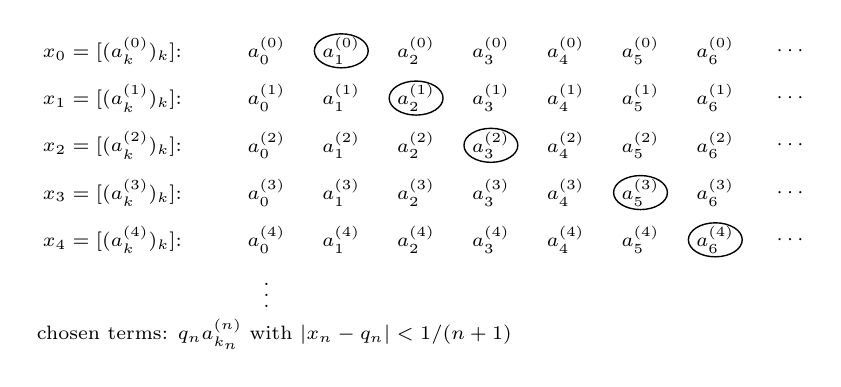
\begin{tikzpicture}[font=\scriptsize, x=0.95cm, y=0.6cm]
\foreach \n in {0,...,4} {
  \node[anchor=east] at (-0.4,-\n) {$x_{\n}=[(a^{(\n)}_k)_k]$:};
  \foreach \k in {0,...,6} {\node at (\k+0.6,-\n) {$a^{(\n)}_{\k}$};}
  \node at (7.6,-\n) {$\cdots$};}
\node at (0.6,-5) {$\vdots$};
\foreach \n/\k in {0/1, 1/2, 2/3, 3/5, 4/6} {\draw[line width=0.5pt] (\k+0.6,-\n) circle (0.36);}
\node[anchor=west] at (-2.6,-6.0) {chosen terms: $q_n\coloneqq a^{(n)}_{k_n}$ with $|x_n-q_n|<1/(n+1)$};
\end{tikzpicture}}{The proof of \cref{thm:r-cauchy-complete}. Row $n$ lists a representative of the real number $x_n$, a Cauchy sequence of rational numbers that converges to $x_n$ by \cref{thm:r-archimedean}. In each row a term $q_n$ (circled) is chosen so close to $x_n$ that the rational numbers $q_0,q_1,\ldots$ form a Cauchy sequence; its class is the limit of $(x_n)$.\label{fig:diagonal}}
\end{figure}

\begin{theorem}[Cauchy completeness]
\label{thm:r-cauchy-complete}
Every Cauchy sequence in $\mathbb R$ converges in $\mathbb R$.
\end{theorem}

\begin{proof}
Let $(x_n)$ be a Cauchy sequence in $\mathbb R$. For each $n$, choose a representative $a^{(n)}\in\mathcal C$ of $x_n$. By \cref{thm:r-archimedean}\,(ii), $a^{(n)}_k\to x_n$ as $k\to\infty$, so there is an index $k_n$ with $|x_n-a^{(n)}_{k_n}|<1/(n+1)$; put $q_n\coloneqq a^{(n)}_{k_n}\in\mathbb Q$.

The sequence $q=(q_n)$ is a Cauchy sequence in $\mathbb Q$. Let $\varepsilon>0$ be rational, and choose $N$ with $1/(N+1)<\varepsilon/3$ and $|x_m-x_n|<\varepsilon/3$ for all $m,n\ge N$. For $m,n\ge N$,
\[
|q_m-q_n|\le|q_m-x_m|+|x_m-x_n|+|x_n-q_n|<\frac1{m+1}+\frac\varepsilon3+\frac1{n+1}<\varepsilon .
\]
This is an inequality between real numbers, but its two ends are rational, and the order of $\mathbb R$ restricted to $\mathbb Q$ is the order of $\mathbb Q$ (\cref{thm:r-ordered}); so $|q_m-q_n|<\varepsilon$ holds in $\mathbb Q$.

Let $x\coloneqq[q]$. By \cref{thm:r-archimedean}\,(ii), $q_n\to x$ in $\mathbb R$, and therefore
\[
|x_n-x|\le|x_n-q_n|+|q_n-x|<\frac1{n+1}+|q_n-x|\to0 ,
\]
using $1/(n+1)\to0$ in the Archimedean field $\mathbb R$ (\cref{prop:archimedean-forms}). So $x_n\to x$.
\end{proof}

The choice of the indices $k_n$ is a kind of diagonal argument through the table of representatives in \cref{fig:diagonal}, with one term picked from each row. The second form of completeness, the one that Volume~I took as its axiom, now follows by bisection, with rational endpoints.

\begin{theorem}[Least upper bound property]
\label{thm:r-sup}
Every nonempty subset of $\mathbb R$ that is bounded above has a supremum in $\mathbb R$.
\end{theorem}

\begin{proof}
Let $S\subseteq\mathbb R$ be nonempty and bounded above. We construct rational numbers $a_k$ and $b_k$ such that, for every $k$, $a_k$ is not an upper bound of $S$, $b_k$ is an upper bound of $S$, and $b_k-a_k=(b_0-a_0)/2^k$. To start, choose $s\in S$ and an upper bound $u$ of $S$, and, by \cref{thm:r-archimedean}\,(i), rational numbers $a_0<s$ and $b_0>u$. Given $a_k$ and $b_k$, let $m_k\coloneqq(a_k+b_k)/2$, again rational. If $m_k$ is an upper bound of $S$, put $a_{k+1}\coloneqq a_k$ and $b_{k+1}\coloneqq m_k$; otherwise put $a_{k+1}\coloneqq m_k$ and $b_{k+1}\coloneqq b_k$. The three properties are preserved, and in both cases $a_k\le a_{k+1}<b_{k+1}\le b_k$.

For $m,n\ge k$ both $a_m$ and $a_n$ lie in $[a_k,b_k]$, so $|a_m-a_n|\le b_k-a_k=(b_0-a_0)/2^k$, and the same holds for $(b_n)$. Since $2^k\ge k+1$ and $\mathbb Q$ is Archimedean, $(b_0-a_0)/2^k\to0$; hence $a=(a_k)$ and $b=(b_k)$ belong to $\mathcal C$, and $b-a$ is a null sequence. Let $\sigma\coloneqq[a]=[b]$.

By \cref{thm:r-archimedean}\,(ii), $a_k\to\sigma$ and $b_k\to\sigma$ in $\mathbb R$. If $x\in S$, then $x\le b_k$ for every $k$, so $x\le\sigma$ by \cref{prop:of-limits}\,(iv); thus $\sigma$ is an upper bound of $S$. If $v<\sigma$, then $a_k>v$ for some $k$, by \cref{prop:of-limits}\,(iv) applied to the constant sequence $v$; since $a_k$ is not an upper bound, some $x\in S$ satisfies $x>a_k>v$, and $v$ is not an upper bound either. So $\sigma$ is the least upper bound of $S$.
\end{proof}

\begin{theorem}[Existence of the real numbers]
\label{thm:reals-exist}
The field $\mathbb R$ of \cref{def:real-numbers-cauchy}, ordered by \cref{def:real-positive}, is a complete ordered field. In particular, \vcref{1}{asm:reals} holds.
\end{theorem}

\begin{proof}
$\mathbb R$ is an ordered field by \cref{thm:r-ordered}, and it is complete in the sense of \vcref{1}{def:complete} by \cref{thm:r-sup}.
\end{proof}

By \cref{thm:uniqueness-complete} below, any complete ordered field is a copy of this one, by an isomorphism that preserves everything in sight, and there is only one such isomorphism. We may therefore, and from now on do, regard the field constructed here as the field $\mathbb R$ of Volumes~I and~II. Every theorem proved there from \vcref{1}{asm:reals} holds for it, and we cite those theorems freely: the monotone convergence theorem, the nested interval theorem, the Bolzano--Weierstrass theorem, the Cauchy criterion, and everything built on them. The circle of definitions is closed as well. \Vcref{1}{def:cauchy} defined Cauchy sequences of real numbers, and \cref{thm:r-cauchy-complete} is the half of the Cauchy criterion \vcref{1}{thm:cauchy-criterion} that Volume~I deduced from the Bolzano--Weierstrass theorem; here it has been proved directly from the construction.

The logical position is now the following. Peano's axioms describe $\mathbb N$; in axiomatic set theory a set satisfying them exists by the axiom of infinity, as \vcref{1}{sec:naturals} explains. From $\mathbb N$ one constructs $\mathbb Z$ and $\mathbb Q$ by classes of pairs, and from $\mathbb Q$ one constructs $\mathbb R$ by classes of Cauchy sequences, and $\mathbb C$ as pairs of real numbers (\vcref{1}{sec:complex}). Every number system of Volumes~I and~II is thereby reduced to the natural numbers, and its consistency to the consistency of set theory.

\subsection{Expansions}

\Vcref{1}{thm:real-expansion} showed that every real number $x\in[0,1)$ has a base-$b$ expansion whose truncations $s_m=\lfloor b^mx\rfloor/b^m$ satisfy $s_m\le x<s_m+b^{-m}$. The truncations are rational and converge to $x$, so by \cref{thm:r-archimedean}\,(iii) the sequence $(s_m)$ is one of the representatives of $x$. The expansion thus singles out a canonical representative in each class, and one could try to define the real numbers as expansions, a real number being an infinite string of digits. This is the picture of the real numbers that most of us carry from school, and it is not wrong; but it is awkward as a definition. The numbers with two expansions, such as $1=(0.\overline9)_{10}$, must be identified by hand, and the arithmetic of infinite strings is unpleasant: to add $(0.333\ldots)_{10}$ and $(0.666\ldots)_{10}$, or to multiply $(0.333\ldots)_{10}$ by $3$, one must know whether a carry will ever arrive from far to the right, which no finite inspection of the digits decides. The construction by classes avoids these difficulties by allowing all Cauchy sequences, not only truncations, as representatives, and the price is only that a real number becomes a class rather than a single sequence.

\section{Dedekind Cuts}
\label{sec:dedekind}

Dedekind's construction, published in the same year as Cantor's, starts from the picture of \vcref{1}{fig:sup-cut}B: a gap of $\mathbb Q$ divides the rational numbers into those below it and those above it, and the lower part determines the gap. Dedekind declared the lower part itself to be the new number~\cite{dedekind1872}. Only the order of $\mathbb Q$ is needed for the definition; arithmetic enters only afterwards.

\begin{definition}[Dedekind cut]
\label{def:cut}
A \term{cut} is a subset $\alpha\subseteq\mathbb Q$ with the following properties:
\begin{enumerate}
\item $\alpha\ne\emptyset$ and $\alpha\ne\mathbb Q$;
\item $\alpha$ is closed downwards: if $p\in\alpha$ and $q<p$, then $q\in\alpha$;
\item $\alpha$ has no greatest element.
\end{enumerate}
For $r\in\mathbb Q$ the cut $r^*\coloneqq\{q\in\mathbb Q: q<r\}$ is the \term{rational cut} of $r$. Cuts are ordered by inclusion: $\alpha\le\beta$ means $\alpha\subseteq\beta$.
\end{definition}

The set $r^*$ is a cut: it contains $r-1$, it does not contain $r$, it is closed downwards, and for $q\in r^*$ the element $(q+r)/2$ of $r^*$ is larger. The set $A=\{x\in\mathbb Q: x\le0\text{ or }x^2<2\}$ of \vcref{1}{prop:q-gap} is a cut as well. It contains $1$ and not $2$; if $x\in A$ and $q<x$, then either $q\le0$, or $0<q<x$ and $q^2<x^2<2$, so $q\in A$; and $A$ has no greatest element, because $1\in A$ exceeds every $x\le0$, and the proof of that proposition produced for every $x\in A$ with $x>0$ an element $f(x)>x$ of $A$. It is not a rational cut, because a rational cut $r^*$ has the supremum $r$ in $\mathbb Q$ and $A$ has none. The condition (iii) is a normalisation: without it, both $\{q: q<r\}$ and $\{q: q\le r\}$ would represent $r$.

\begin{proposition}
\label{prop:cut-order}
The relation $\le$ is a total order on the set of cuts, and $r<s$ implies $r^*<s^*$.
\end{proposition}

\begin{proof}
Inclusion is reflexive, antisymmetric and transitive. Let $\alpha$ and $\beta$ be cuts with $\alpha\not\subseteq\beta$, and choose $p\in\alpha\setminus\beta$. For every $q\in\beta$ we have $q<p$, since $q\ge p$ would put $p$ into $\beta$ by (ii); hence $q\in\alpha$ by (ii) for $\alpha$. So $\beta\subseteq\alpha$, and any two cuts are comparable. If $r<s$, then $r^*\subseteq s^*$, and $r\in s^*\setminus r^*$.
\end{proof}

\begin{theorem}[Completeness of the cuts]
\label{thm:cut-sup}
Let $\mathcal A$ be a nonempty set of cuts that is bounded above by a cut $\beta$. Then the union $\gamma\coloneqq\bigcup_{\alpha\in\mathcal A}\alpha$ is a cut, and it is the supremum of $\mathcal A$.
\end{theorem}

\begin{proof}
$\gamma$ is nonempty because $\mathcal A$ is nonempty and its members are; $\gamma\ne\mathbb Q$ because $\gamma\subseteq\beta\ne\mathbb Q$. If $p\in\gamma$, then $p\in\alpha$ for some $\alpha\in\mathcal A$; every $q<p$ lies in $\alpha\subseteq\gamma$, and $\alpha$ contains an element larger than $p$, which lies in $\gamma$. So $\gamma$ is a cut. It contains every $\alpha\in\mathcal A$, so it is an upper bound, and every upper bound $\delta$ of $\mathcal A$ contains every $\alpha$ and hence $\gamma$.
\end{proof}

So completeness, which cost the whole of \cref{sec:completeness-proof} for Cauchy sequences, is almost free for cuts. The price is paid in the arithmetic. Sums are still simple, but negatives and products are not, because the lower part of $-x$ is the negative of the \emph{upper} part of $x$, and multiplying by a negative number exchanges lower and upper parts.

\begin{definition}[Arithmetic of cuts]
\label{def:cut-arithmetic}
For cuts $\alpha$ and $\beta$ let
\begin{gather*}
\alpha+\beta\coloneqq\{p+q: p\in\alpha,\ q\in\beta\},\\
-\alpha\coloneqq\{p\in\mathbb Q:\ -p-r\notin\alpha\text{ for some rational }r>0\}.
\end{gather*}
If $\alpha>0^*$ and $\beta>0^*$, let $\alpha\beta\coloneqq\{p\in\mathbb Q: p\le rs\text{ for some }r\in\alpha,\ s\in\beta\text{ with }r>0,\ s>0\}$. In the remaining cases, let $\alpha0^*\coloneqq0^*\alpha\coloneqq0^*$, and
\[
\alpha\beta\coloneqq\begin{cases}(-\alpha)(-\beta)&\text{if }\alpha<0^*\text{ and }\beta<0^*,\\ -\bigl((-\alpha)\beta\bigr)&\text{if }\alpha<0^*<\beta,\\ -\bigl(\alpha(-\beta)\bigr)&\text{if }\beta<0^*<\alpha.\end{cases}
\]
\end{definition}

In the definition of $-\alpha$, the number $-p$ is required to lie strictly beyond the upper part of $\alpha$, by some positive margin $r$; the margin ensures that $-\alpha$ has no greatest element when $\alpha$ is a rational cut. For $\alpha=r^*$ one finds $-\alpha=(-r)^*$, as it should be.

\begin{theorem}[Dedekind]
\label{thm:cuts-field}
With the operations of \cref{def:cut-arithmetic} and the order by inclusion, the set of cuts is a complete ordered field. Its zero is $0^*$, its one is $1^*$, its positive elements are the cuts $\alpha>0^*$, and its rational elements are the rational cuts: $r\mapsto r^*$ is the map $\iota$ of \cref{prop:prime-field}.
\end{theorem}

\begin{proof}[sketch]
Completeness is \cref{thm:cut-sup}, and the order is total by \cref{prop:cut-order}. One checks first that the sets $\alpha+\beta$, $-\alpha$ and $\alpha\beta$ are cuts, which is a direct verification of the three conditions of \cref{def:cut}. Commutativity and associativity of addition are inherited from $\mathbb Q$. For $\alpha+0^*=\alpha$: every $p+q$ with $p\in\alpha$ and $q<0$ is smaller than $p$ and therefore lies in $\alpha$; conversely, for $p\in\alpha$ choose a larger $p'\in\alpha$, and then $p=p'+(p-p')$ with $p-p'<0$. The identity $\alpha+(-\alpha)=0^*$ is the first place where more than the order of $\mathbb Q$ is needed. Given a rational $v<0$, put $w\coloneqq-v/2$. Since $\alpha$ is nonempty and bounded above, and $\mathbb Q$ is Archimedean, there is an integer $n$ with $nw\in\alpha$ and $(n+1)w\notin\alpha$; then $-(n+2)w\in-\alpha$, with the margin $r=w$, and $nw+\bigl(-(n+2)w\bigr)=v$. So $0^*\subseteq\alpha+(-\alpha)$, and the reverse inclusion follows from the definition of $-\alpha$. The multiplicative axioms are first proved for positive cuts, where the same kind of argument works, with the Archimedean property used to find the inverse; they are then extended to all cuts through the case distinction of \cref{def:cut-arithmetic}, and the distributive law in particular requires working through the cases of signs. The axioms of order follow from the definitions of the sum and of the product of positive cuts, and the rational cuts are added and multiplied like the rational numbers. Rudin carries out all these verifications in the appendix to the first chapter of his book~\cite{rudin1976}, and Landau's \emph{Grundlagen} does it starting from the natural numbers~\cite{landau1930}.
\end{proof}

\Cref{tab:two-constructions} compares the two constructions. In Cantor's, the algebra is easy and completeness is the main theorem; in Dedekind's, completeness is immediate and the algebra is laborious. By \cref{thm:uniqueness-complete} below they produce the same field, and \cref{sec:uniqueness} writes down the isomorphism between them. There is a reason for preferring Cauchy sequences in this series. Dedekind's construction uses the order of $\mathbb Q$ and nothing else, so it generalises to ordered sets: every partially ordered set can be embedded into one in which every subset has a supremum and an infimum, its \emph{Dedekind--MacNeille completion}~\cite{daveypriestley2002}. Cantor's construction uses the distance $|p-q|$ and the arithmetic, not the order, so it generalises to sets in which distances are defined but no order is. The next chapter completes in this way every metric space, and Part~III shows that the spaces $L^p$ of integrable functions are the completions, in this sense, of spaces of continuous functions with a distance given by an integral. The rational numbers are the first example of an incomplete space whose completion is wanted, and the real numbers the first completion.

\begin{table}
\sdfloat{%
\begin{sdtable}{colspec={lll}, row{1}={font=\small\bfseries}}
\toprule
 & Cauchy sequences (Cantor) & cuts (Dedekind) \\
\midrule
a real number is & a class of Cauchy sequences in $\mathbb Q$ & a lower part of $\mathbb Q$ \\
uses of $\mathbb Q$ & arithmetic and distance & order \\
sum and product & termwise & sum by elements, product by cases \\
$x<y$ & terms eventually apart by some $\delta>0$ & proper inclusion \\
completeness & \cref{thm:r-cauchy-complete,thm:r-sup} & the union, \cref{thm:cut-sup} \\
generalises to & completion of metric spaces & completion of ordered sets \\
\bottomrule
\end{sdtable}}{The two classical constructions of the real numbers from $\mathbb Q$. They produce isomorphic complete ordered fields, by \cref{thm:uniqueness-complete}.\label{tab:two-constructions}}
\end{table}

\section{Uniqueness}
\label{sec:uniqueness}

\Vcref{1}{thm:r-unique} asserted that a complete ordered field is unique: between two of them there is exactly one bijection that preserves sums and products, and it preserves the order. Volume~I gave the storyline of the proof. We now prove the theorem, and in a stronger form that also describes the ordered fields that are not complete but Archimedean. Two facts about complete ordered fields come first.

\begin{lemma}
\label{lem:complete-basic}
Let $F$ be a complete ordered field.
\begin{enumerate}
\item $F$ is Archimedean, and its rational elements are dense in $F$.
\item Every $x\ge0$ in $F$ is the square of exactly one $y\ge0$ in $F$. Consequently the elements $x\ge0$ of $F$ are exactly the squares.
\end{enumerate}
\end{lemma}

\begin{proof}
(i) The proof of \vcref{1}{thm:archimedes} uses only the approximation property of the supremum, \vcref{1}{lem:sup-approx}, whose proof uses only the order, and the existence of suprema; it is valid in $F$. Density follows by \cref{prop:archimedean-forms}.

(ii) The proof of \vcref{1}{thm:roots}, for $n=2$, uses the axioms of an ordered field, the existence of a supremum, and the choice of elements $h$ and $k$ by field operations; it is valid in $F$. Conversely every square is nonnegative, by \vcref{1}{prop:order-rules}\,(iv).
\end{proof}

The main theorem compares an Archimedean field with a complete one. For two ordered fields $F$ and $F'$, a map $\varphi\colon F\to F'$ \term{preserves sums, products and order} if $\varphi(x+y)=\varphi(x)+\varphi(y)$, $\varphi(xy)=\varphi(x)\varphi(y)$, and $x\le y$ implies $\varphi(x)\le\varphi(y)$; as in \cref{sec:ordered-fields}, $q'$ denotes the rational element of $F'$ that corresponds to the rational element $q$ of $F$.

\begin{theorem}[Embedding of Archimedean fields]
\label{thm:archimedean-embedding}
Let $F$ be an Archimedean ordered field and $F'$ a complete ordered field. There is exactly one map $\varphi\colon F\to F'$ that preserves sums, products and order and satisfies $\varphi(1)=1$. It is given by
\begin{equation}
\varphi(x)=\sup\{q': q\in\mathbb Q,\ q<x\}\qquad(x\in F),
\label{eq:embedding-sup}
\end{equation}
it maps each rational element $q$ of $F$ to $q'$, and it is strictly increasing, in particular injective. If $F$ is complete as well, $\varphi$ is a bijection.
\end{theorem}

\begin{proof}
\emph{A characterisation.} For $x\in F$, let $L_x$ and $U_x$ be the sets of rational $q$ with $q<x$ and with $q>x$; both are nonempty, since $F$ is Archimedean. We claim that there is exactly one $z\in F'$ with
\begin{equation}
q'\le z\le r'\qquad\text{for all }q\in L_x\text{ and }r\in U_x .
\label{eq:squeeze-rationals}
\end{equation}
For existence, $q<x<r$ gives $q'<r'$, so each $r'$ with $r\in U_x$ is an upper bound of $\{q': q\in L_x\}$; the supremum $z$ of this set exists in $F'$ and satisfies \eqref{eq:squeeze-rationals}. For uniqueness, suppose that $z_1<z_2$ both satisfy \eqref{eq:squeeze-rationals}. Since $F'$ is complete, its rational elements are dense (\cref{lem:complete-basic}), and there are rational $s<t$ with $z_1<s'<t'<z_2$. At least one of $s$ and $t$, call it $u$, differs from $x$. If $u<x$, then $u\in L_x$ and $u'\le z_1$, contradicting $z_1<s'\le u'$; if $u>x$, then $u\in U_x$ and $z_2\le u'$, contradicting $u'\le t'<z_2$. We define $\varphi(x)$ as this $z$; thus \eqref{eq:embedding-sup} holds.

\emph{Rational elements.} For rational $q$, the element $q'$ satisfies \eqref{eq:squeeze-rationals} for $x=q$, by \cref{prop:prime-field}; so $\varphi(q)=q'$, and in particular $\varphi(0)=0$ and $\varphi(1)=1$.

\emph{Order.} If $x<y$ in $F$, density in $F$ (\cref{prop:archimedean-forms}) gives rationals $s<t$ with $x<s<t<y$, and then $\varphi(x)\le s'<t'\le\varphi(y)$ by \eqref{eq:squeeze-rationals}. So $\varphi$ is strictly increasing.

\emph{Sums.} Let $x,y\in F$ and $z\coloneqq\varphi(x)+\varphi(y)$. We show that $z$ satisfies \eqref{eq:squeeze-rationals} for $x+y$. Let $u<x+y$ be rational, and put $\delta\coloneqq(x+y-u)/2>0$. Choose rationals $q$ and $q_2$ with $x-\delta<q<x$ and $y-\delta<q_2<y$. Then $u=(x-\delta)+(y-\delta)<q+q_2$, and
\[
u'<q'+q_2'\le\varphi(x)+\varphi(y)=z .
\]
In the same way $z\le w'$ for every rational $w>x+y$. By the uniqueness of $z$ in \eqref{eq:squeeze-rationals}, $\varphi(x+y)=\varphi(x)+\varphi(y)$. It follows that $\varphi(-x)=-\varphi(x)$, since $\varphi(x)+\varphi(-x)=\varphi(0)=0$.

\emph{Products.} Let first $x>0$ and $y>0$, so that $\varphi(x)>0$ and $\varphi(y)>0$, and put $z\coloneqq\varphi(x)\varphi(y)$. Let $u<xy$ be rational. If $u\le0$, then $u'\le0<z$. If $u>0$, then $u/y<x$, and we may choose a rational $q$ with $\max(0,u/y)<q<x$; then $u/q<y$, and we choose a rational $q_2$ with $u/q<q_2<y$. Now $u<qq_2$, and since $0<q'\le\varphi(x)$ and $0<q_2'\le\varphi(y)$,
\[
u'<q'q_2'\le\varphi(x)\varphi(y)=z .
\]
Similarly, if $w>xy$ is rational, choose rationals $r$ and $r_2$ with $x<r<w/y$ and $y<r_2<w/r$; then $rr_2<w$ and $z\le r'r_2'<w'$. Hence $\varphi(xy)=\varphi(x)\varphi(y)$ for $x,y>0$. The other cases follow from this one, from $\varphi(0)=0$ and from $\varphi(-x)=-\varphi(x)$; for instance, if $x<0<y$, then $\varphi(xy)=-\varphi((-x)y)=-\varphi(-x)\varphi(y)=\varphi(x)\varphi(y)$.

\emph{Uniqueness.} Let $\psi\colon F\to F'$ preserve sums, products and order, with $\psi(1)=1$. Its restriction to the rational elements has the three properties of \cref{prop:prime-field}, so $\psi(q)=q'$ for every rational $q$. If $q<x<r$ with $q$ and $r$ rational, then $q'=\psi(q)\le\psi(x)\le\psi(r)=r'$. Thus $\psi(x)$ satisfies \eqref{eq:squeeze-rationals}, and $\psi(x)=\varphi(x)$.

\emph{Surjectivity.} Let $F$ be complete. Then $F'$ is Archimedean by \cref{lem:complete-basic}, and the construction with the roles of $F$ and $F'$ exchanged gives a map $\chi\colon F'\to F$ such that, for every $z\in F'$, the element $x\coloneqq\chi(z)$ satisfies $q\le x\le r$ for all rationals $q,r$ with $q'<z<r'$. We show that $\varphi(x)=z$, by verifying \eqref{eq:squeeze-rationals} for $z$. Let $u<x$ be rational. If $z<u'$, then $u$ would be one of the rationals $r$ with $z<r'$, and $x\le u$ would follow, contradicting $u<x$; hence $u'\le z$. In the same way $z\le w'$ for every rational $w>x$. So $\varphi(\chi(z))=z$ for every $z\in F'$, and $\varphi$ is surjective.
\end{proof}

The formula \eqref{eq:embedding-sup} says that $\varphi(x)$ is determined by the rational numbers below $x$, which is the content of Dedekind's construction: an element of an Archimedean field is fixed by its cut. Taking $F'=\mathbb R$, the theorem shows that every Archimedean ordered field is, up to a unique isomorphism, a subfield of $\mathbb R$ with the order inherited from $\mathbb R$. The uniqueness of complete ordered fields is now a short step.

\begin{theorem}[Uniqueness of the real numbers]
\label{thm:uniqueness-complete}
Let $F$ and $F'$ be complete ordered fields. There is exactly one bijection $\varphi\colon F\to F'$ that preserves sums and products. It preserves the order, and it maps each rational element $q$ of $F$ to $q'$.
\end{theorem}

\begin{proof}
By \cref{lem:complete-basic} $F$ is Archimedean, so \cref{thm:archimedean-embedding} provides a bijection $\varphi$ that preserves sums, products and order and maps $q$ to $q'$. Let $\psi\colon F\to F'$ be any bijection that preserves sums and products. Then $\psi(0)=\psi(0+0)=2\psi(0)$, so $\psi(0)=0$, and $\psi(1)=\psi(1)^2$, so $\psi(1)$ is $0$ or $1$; since $\psi$ is injective and $\psi(0)=0$, $\psi(1)=1$. If $x\ge0$, then $x=y^2$ for some $y$, by \cref{lem:complete-basic}\,(ii), and $\psi(x)=\psi(y)^2\ge0$. Hence $x\le y$ implies $\psi(y)-\psi(x)=\psi(y-x)\ge0$: $\psi$ preserves the order. By the uniqueness part of \cref{thm:archimedean-embedding}, $\psi=\varphi$.
\end{proof}

This is \vcref{1}{thm:r-unique}, and its proof follows the storyline given there: the rational elements are fixed, the order is fixed because the nonnegative elements are the squares, and the supremum of the rational elements below $x$ fixes the image of $x$. With \cref{thm:reals-exist}, it shows that \vcref{1}{asm:reals} describes exactly one structure, up to a unique isomorphism. In particular the field of Cauchy classes and the field of Dedekind cuts are isomorphic, and the isomorphism is explicit: by \eqref{eq:embedding-sup} and \cref{thm:cut-sup}, it maps a real number $x=[a]$ to the union of the rational cuts $q^*$ with $q<x$, which is the cut $\{q\in\mathbb Q: q<x\}$, by the density of $\mathbb Q$ in $\mathbb R$. A real number given by a Cauchy sequence $(a_n)$ thus corresponds to the cut of the rational numbers $q$ for which $a_n-q$ eventually exceeds some positive $\delta$, by \cref{lem:termwise-order}\,(i).

\begin{corollary}
\label{cor:r-automorphism}
Let $f\colon\mathbb R\to\mathbb R$ satisfy $f(x+y)=f(x)+f(y)$ and $f(xy)=f(x)f(y)$ for all $x,y$, and suppose that $f$ is not identically zero. Then $f$ is the identity. In particular, the identity is the only automorphism of the field $\mathbb R$.
\end{corollary}

\begin{proof}
From $f(1)=f(1)^2$ we get $f(1)\in\{0,1\}$, and $f(1)=0$ would give $f(x)=f(x)f(1)=0$ for every $x$. So $f(1)=1$. If $x\ge0$, then $x=y^2$ and $f(x)=f(y)^2\ge0$; as in the proof of \cref{thm:uniqueness-complete}, $f$ preserves the order. By the uniqueness part of \cref{thm:archimedean-embedding} with $F=F'=\mathbb R$, $f$ equals the identity, which is such a map.
\end{proof}

The hypotheses matter, as three examples show. The field $\mathbb C$ has a second automorphism, complex conjugation (\vcref{1}{prop:conjugate}); it has no order, and nothing forces an automorphism to fix $i$ rather than exchange it with $-i$. The field $\mathbb Q(\sqrt2)\coloneqq\{a+b\sqrt2: a,b\in\mathbb Q\}$ is a subfield of $\mathbb R$: it is closed under sums and products, and the inverse of $a+b\sqrt2\ne0$ is $(a-b\sqrt2)/(a^2-2b^2)$, where $a^2\ne2b^2$ because $\sqrt2$ is irrational. Its elements have unique coordinates $a$, $b$, again by the irrationality of $\sqrt2$, and the conjugation $\sigma(a+b\sqrt2)\coloneqq a-b\sqrt2$ preserves sums and products, as one checks from $(a+b\sqrt2)(c+d\sqrt2)=(ac+2bd)+(ad+bc)\sqrt2$. It is not the identity and does not preserve the order, since it maps $\sqrt2>0$ to $-\sqrt2<0$. The argument with squares fails here because $\sqrt2$ is positive but not a square in $\mathbb Q(\sqrt2)$: $(a+b\sqrt2)^2=\sqrt2$ would require $a^2+2b^2=0$ and $2ab=1$. So $\sigma$, followed by the inclusion into $\mathbb R$, is a second embedding of $\mathbb Q(\sqrt2)$ into $\mathbb R$ that preserves sums and products; by \cref{thm:archimedean-embedding}, the inclusion is the only one that also preserves the order.

Finally, the field $\mathbb Q(x)$ of \cref{prop:rational-functions} shows that the Archimedean property of $F$ cannot be dropped from \cref{thm:archimedean-embedding}. The substitution $\tau(p(x)/q(x))\coloneqq p(x+1)/q(x+1)$ is well defined, since $ps=qr$ implies $p(x+1)s(x+1)=q(x+1)r(x+1)$, it preserves sums and products, and it has the inverse $x\mapsto x-1$. It preserves the leading coefficients, so it preserves the order. But it is not the identity, since $\tau(x)=x+1$. The rational elements of $\mathbb Q(x)$ are not dense, and $x$ is not determined by the rational numbers below it: all of them lie below $x$ and below $x+1$ alike. For the same reason $\mathbb Q(x)$ has no order-preserving embedding into $\mathbb R$ at all, which would have to send $x$ to an upper bound of $\mathbb N$.

\section{The Forms of Completeness}
\label{sec:forms-completeness}

Volume~I took the existence of suprema as its completeness axiom and derived from it, in \vcref{1}{ch:limits}, the convergence of bounded monotone sequences, the nested interval theorem, the Bolzano--Weierstrass theorem and the Cauchy criterion. Its note on equivalent forms of completeness stated that each of these can serve as the axiom instead, provided that the Archimedean property is added to the last two, and left the remaining implications to the literature. We now prove the equivalence in an arbitrary ordered field, and show by an example that the Archimedean hypothesis cannot be omitted. In an ordered field $F$, a \term{closed bounded interval} is a set $[a,b]\coloneqq\{x\in F: a\le x\le b\}$ with $a\le b$ in $F$, and its \term{length} is $b-a$; a sequence of intervals $I_n=[a_n,b_n]$ is \term{nested} if $I_{n+1}\subseteq I_n$ for every $n$.

\begin{theorem}[Forms of completeness]
\label{thm:completeness-forms}
For an ordered field $F$ the following statements are equivalent.
\begin{enumerate}
\item[(a)] $F$ is complete: every nonempty subset of $F$ that is bounded above has a supremum.
\item[(b)] Every increasing sequence in $F$ that is bounded above converges.
\item[(c)] $F$ is Archimedean, and every nested sequence of closed bounded intervals in $F$ has a nonempty intersection.
\item[(d)] Every bounded sequence in $F$ has a convergent subsequence.
\item[(e)] $F$ is Archimedean, and every Cauchy sequence in $F$ converges.
\end{enumerate}
Moreover, (c) remains equivalent to the other statements if the nonempty intersection is required only for nested sequences of closed bounded intervals whose lengths tend to zero; we call this weaker statement (c$'$).
\end{theorem}

\begin{proof}
We prove (a)$\Rightarrow$(b)$\Rightarrow$(c)$\Rightarrow$(c$'$)$\Rightarrow$(a) and (c$'$)$\Rightarrow$(d)$\Rightarrow$(e)$\Rightarrow$(c$'$); \cref{fig:completeness-implications} shows the scheme.

(a)$\Rightarrow$(b): the proof of the monotone convergence theorem, \vcref{1}{thm:monotone}, uses only the approximation property of the supremum and is valid in $F$.

(b)$\Rightarrow$(c): suppose first that $\mathbb N$ were bounded above in $F$. Then the increasing sequence $(n)_{n\in\mathbb N}$ would converge, by (b), and so it would be a Cauchy sequence (\cref{prop:of-limits}\,(ii)); but $|(n+1)-n|=1$ for every $n$, so the tolerance $1$ is never met. Hence $F$ is Archimedean. Now let $I_n=[a_n,b_n]$ be nested. As at the beginning of the proof of \vcref{1}{thm:nested}, $a_n\le a_{n+1}\le b_{n+1}\le b_n$, and $a_n\le b_m$ for all $m$ and $n$. So $(a_n)$ is increasing and bounded above by $b_0$, and it converges to some $\alpha\in F$ by (b). For each $n$, $a_n\le a_k\le b_n$ for all $k\ge n$, so $a_n\le\alpha\le b_n$ by \cref{prop:of-limits}\,(iv). Thus $\alpha$ lies in every $I_n$.

(c)$\Rightarrow$(c$'$) is trivial.

(c$'$)$\Rightarrow$(a): let $S$ be nonempty and bounded above, $s\in S$ and $u$ an upper bound. Put $a_0\coloneqq s-1$, which is not an upper bound, and $b_0\coloneqq u$, and bisect as in the proof of \cref{thm:r-sup}: if the midpoint $m_k$ of $[a_k,b_k]$ is an upper bound of $S$, let $[a_{k+1},b_{k+1}]\coloneqq[a_k,m_k]$, and otherwise $[a_{k+1},b_{k+1}]\coloneqq[m_k,b_k]$. Then each $a_k$ is not an upper bound, each $b_k$ is one, and the intervals are nested with lengths $(b_0-a_0)/2^k$, which tend to zero because $2^k\ge k+1$ and $F$ is Archimedean (\cref{prop:archimedean-forms}). By (c$'$) there is $\sigma$ in all of them. Then $0\le b_k-\sigma\le b_k-a_k$ and $0\le\sigma-a_k\le b_k-a_k$, so $a_k\to\sigma$ and $b_k\to\sigma$. Every $x\in S$ satisfies $x\le b_k$ for all $k$, hence $x\le\sigma$; and if $v<\sigma$, then $a_k>v$ for some $k$, and since $a_k$ is not an upper bound, neither is $v$. So $\sigma=\sup S$.

(c$'$)$\Rightarrow$(d): this is the second proof of the Bolzano--Weierstrass theorem in \vcref{1}{ch:limits}, after \vcref{1}{thm:bolzano-weierstrass}. Let $|x_n|\le C$ for all $n$, and $I_0\coloneqq[-C,C]$. Recursively, let $I_{k+1}$ be a half of $I_k$ that contains $x_n$ for infinitely many indices $n$; one of the two halves does, because $I_k$ does. The lengths $2C/2^k$ tend to zero, since $F$ is Archimedean, and (c$'$) provides a point $x$ in every $I_k$. Choose indices $n_0<n_1<\cdots$ with $x_{n_k}\in I_k$, which is possible because each $I_k$ contains terms with arbitrarily large indices. Then $|x_{n_k}-x|\le2C/2^k\to0$.

(d)$\Rightarrow$(e): if $\mathbb N$ were bounded above, the sequence $(n)$ would be bounded, and by (d) it would have a convergent subsequence $(n_k)$; but $|n_{k+1}-n_k|\ge1$ for every $k$, so this subsequence is not a Cauchy sequence, a contradiction. So $F$ is Archimedean. A Cauchy sequence is bounded (\cref{prop:of-limits}\,(ii)), so by (d) it has a convergent subsequence, and then it converges itself, by \cref{prop:of-limits}\,(vi). This is the proof of \vcref{1}{thm:cauchy-criterion}.

(e)$\Rightarrow$(c$'$): let $I_n=[a_n,b_n]$ be nested with $b_n-a_n\to0$. For $m,n\ge k$ both $a_m$ and $a_n$ lie in $I_k$, so $|a_m-a_n|\le b_k-a_k$, and $(a_n)$ is a Cauchy sequence. By (e) it converges to some $\alpha$, and as in the proof of (b)$\Rightarrow$(c), $\alpha$ lies in every $I_n$.
\end{proof}

\begin{figure}
\sdfloat{%
\begin{tikzpicture}[font=\scriptsize,
  box/.style={draw, line width=0.4pt, align=center, text width=2.55cm, minimum height=0.95cm, inner sep=2pt},
  old/.style={-{Latex[length=1.6mm]}, line width=0.5pt},
  new/.style={-{Latex[length=1.6mm]}, line width=0.5pt, dashed}]
\node[box] (a) at (0,1.9) {(a) suprema};
\node[box] (b) at (3.4,1.9) {(b) monotone limits};
\node[box] (c) at (6.8,1.9) {(c) nested intervals,\\ Archimedean};
\node[box] (cp) at (6.8,0) {(c$'$) shrinking nested\\ intervals, Archimedean};
\node[box] (d) at (3.4,0) {(d) convergent\\ subsequences};
\node[box] (e) at (0,0) {(e) Cauchy sequences,\\ Archimedean};
\draw[old] (a) -- (b);
\draw[old] (b) -- (c);
\draw[old] (c) -- (cp);
\draw[old] (cp) -- (d);
\draw[old] (d) -- (e);
\draw[new] (e.south) to[out=-25, in=-155] (cp.south);
\draw[new] (cp.north west) -- (a.south east);
\end{tikzpicture}}{The scheme of the proof of \cref{thm:completeness-forms}. Solid arrows follow proofs of Volume~I, read in an arbitrary ordered field (the step from (c) to (c$'$) is trivial); dashed arrows are proved here, and so is the Archimedean property in the steps from (b) to (c) and from (d) to (e). The field of formal Laurent series (\cref{thm:laurent-complete}) satisfies the non-Archimedean part of (c$'$) and of (e), but none of the five statements.\label{fig:completeness-implications}}
\end{figure}

The proof shows that (a), (b) and (d) imply the Archimedean property by themselves, while in (c), (c$'$) and (e) it is a separate hypothesis. It cannot be dropped from (c$'$) and (e). The example is a field of series, which contains infinitesimals in the same way as $\mathbb Q(x)$ but is large enough for every Cauchy sequence to have a limit. Let $K$ be an ordered field; the cases $K=\mathbb Q$ and $K=\mathbb R$ are the ones to keep in mind. A \term{formal Laurent series} over $K$ is an expression
\[
a=\sum_{j\in\mathbb Z}a_jt^j\qquad(a_j\in K),
\]
in which only finitely many coefficients with negative index are nonzero: there is an integer $m$ with $a_j=0$ for all $j<m$. Formally, $a$ is the function $j\mapsto a_j$ from $\mathbb Z$ to $K$, and $t$ is a symbol; nothing is summed. The set of these series is denoted $K((t))$. For $a\ne0$, the least $j$ with $a_j\ne0$ is the \term{order} $v(a)$ of $a$, and $a_{v(a)}$ is its \term{lowest coefficient}. Series are added coefficientwise, and multiplied by
\[
(ab)_j\coloneqq\sum_{i\in\mathbb Z}a_ib_{j-i},
\]
a sum with finitely many nonzero terms: if $a_i=0$ for $i<m$ and $b_k=0$ for $k<m'$, only the indices $m\le i\le j-m'$ contribute. In particular $(ab)_j=0$ for $j<v(a)+v(b)$, and $(ab)_{v(a)+v(b)}=a_{v(a)}b_{v(b)}\ne0$, so $v(ab)=v(a)+v(b)$. We write $t^k$ for the series with the coefficient $1$ at $k$ and $0$ elsewhere, and identify $c\in K$ with $ct^0$.

\begin{theorem}[A complete field that is not Archimedean]
\label{thm:laurent-complete}
Let $K$ be an ordered field. With the operations above, $K((t))$ is a field, and it becomes an ordered field if a nonzero series is declared positive when its lowest coefficient is positive. In this field every Cauchy sequence converges, and every nested sequence of closed bounded intervals whose lengths tend to zero has a nonempty intersection; but the field is not Archimedean: $t^{-1}>n$ for every $n\in\mathbb N$.
\end{theorem}

\begin{proof}
\emph{Field.} The ring axioms are verified as for polynomials: each coefficient of a sum or product of series is a finite expression in finitely many coefficients of the factors, and the identities needed, such as $\bigl((ab)c\bigr)_j=\sum_{i+k+l=j}a_ib_kc_l=\bigl(a(bc)\bigr)_j$, hold in $K$. The one is $t^0$. For the inverse of $a\ne0$, let $m\coloneqq v(a)$ and $u_j\coloneqq a_{j+m}$, so that $a=t^mu$ with $u=\sum_{j\ge0}u_jt^j$ and $u_0\ne0$. Define $w_0\coloneqq1/u_0$ and, recursively,
\[
w_j\coloneqq-\frac1{u_0}\sum_{i=1}^{j}u_iw_{j-i}\qquad(j\ge1),
\]
and $w_j\coloneqq0$ for $j<0$. Then $(uw)_0=u_0w_0=1$, and for $j\ge1$, $(uw)_j=u_0w_j+\sum_{i=1}^ju_iw_{j-i}=0$. So $uw=1$, and $a^{-1}=t^{-m}w$.

\emph{Order.} Let $P$ be the set of nonzero series with positive lowest coefficient. Since $(-a)_{v(a)}=-a_{v(a)}$, exactly one of $a\in P$, $a=0$, $-a\in P$ holds. If $a,b\in P$, the lowest coefficient of $ab$ is $a_{v(a)}b_{v(b)}>0$. For $a+b$: if $v(a)\ne v(b)$, its lowest coefficient is that of the summand of smaller order; if $v(a)=v(b)$, it is $a_{v(a)}+b_{v(b)}$, a sum of two positive elements. In both cases it is positive. So $K((t))$ is an ordered field. Since $t^{-1}-n$ has the lowest coefficient $1$, at the index $-1$, $t^{-1}>n$ for every $n\in\mathbb N$, and the field is not Archimedean.

\emph{Distances and orders.} For $a\ne0$, the series $|a|$ equals $a$ or $-a$, so it has the order $v(a)$ and the lowest coefficient $|a_{v(a)}|>0$. For every integer $k$:
\begin{enumerate}
\item if $v(a)>k$, then $|a|<t^k$, because $t^k-|a|$ has the lowest coefficient $1$ at $k$;
\item if $|a|<t^k$, then $v(a)\ge k$, because for $v(a)<k$ the lowest coefficient of $t^k-|a|$ is $-|a_{v(a)}|<0$;
\item every $\varepsilon>0$ exceeds some $t^k$: with $m\coloneqq v(\varepsilon)$, the series $\varepsilon-t^{m+1}$ has the lowest coefficient $\varepsilon_m>0$; moreover $t^l<t^k$ for $l>k$, since $t^k-t^l$ has the lowest coefficient $1$.
\end{enumerate}
By (i) and (ii), $|a-b|<t^k$ forces $a$ and $b$ to have the same coefficients at all indices $j<k$; by (i), if they have the same coefficients at all $j\le k$, then $|a-b|<t^k$.

\emph{Cauchy sequences converge.} Let $(a_n)$ be a Cauchy sequence. For each integer $k\ge1$ choose $N_k$ with $|a_m-a_n|<t^k$ for all $m,n\ge N_k$, with $N_1\le N_2\le\cdots$. Then all $a_n$ with $n\ge N_k$ have the same coefficients at the indices $j<k$. Define $c_j$, for $j\in\mathbb Z$, as the coefficient of $t^j$ in $a_{N_k}$ for any $k\ge1$ with $k>j$; it does not depend on the choice of $k$, since $a_{N_k}$ and $a_{N_{k'}}$ agree at the indices below $\min(k,k')$. The coefficients $c_j$ with $j<1$ are those of $a_{N_1}$, so they vanish for all sufficiently negative $j$, and $c\coloneqq\sum_jc_jt^j$ belongs to $K((t))$. If $n\ge N_k$, then $a_n$ and $c$ have the same coefficients at all indices $j<k$, so $|a_n-c|<t^{k-1}$. Given $\varepsilon>0$, choose by (iii) an integer $k\ge1$ with $t^{k-1}<\varepsilon$; then $|a_n-c|<\varepsilon$ for all $n\ge N_k$. So $a_n\to c$.

\emph{Shrinking nested intervals.} The proof of (e)$\Rightarrow$(c$'$) in \cref{thm:completeness-forms} used the Archimedean property only as part of the hypothesis, not in the argument; it shows that the convergence of Cauchy sequences alone gives a point in every nested sequence of closed bounded intervals whose lengths tend to zero.
\end{proof}

In $K((t))$ the element $t$ is a positive infinitesimal, and $t^{-1}$ is infinitely large, as in $\mathbb Q(x)$; in fact $\mathbb Q(x)$ sits inside $\mathbb Q((t))$ if $x$ is read as $t^{-1}$, with the same order, since a polynomial $p(t^{-1})$ of degree $d$ is $t^{-d}$ times a series with the constant term $\operatorname{lc}(p)$. The quotient of two such series has the lowest coefficient $\operatorname{lc}(p)/\operatorname{lc}(q)$, whose sign is that of $\operatorname{lc}(p)\operatorname{lc}(q)$. What $K((t))$ has in addition are limits for all its Cauchy sequences; the partial sums $\sum_{j=0}^nt^{j^2}$, for instance, form a Cauchy sequence by (i) of the proof, and their limit is the series with the coefficient $1$ at the squares and $0$ elsewhere. The tolerances that test convergence are the powers $t^k$, which tend to zero; the tolerances $1/n$ do not, and this is why the field is not Archimedean although its Cauchy sequences converge. The field is not complete either: $\mathbb N$ is bounded above by $t^{-1}$ and has no supremum, as in $\mathbb Q(x)$. And for $K=\mathbb Q$ or $K=\mathbb R$, even the full statement (c) fails: the intervals $[n,\,t^{-1}/(n+1)]$ are nested, but a common point $y$ would be larger than every $n$, so $v(y)\le-1$, and at most $t^{-1}/(n+1)$ for every $n$, which forces $v(y)=-1$ and a coefficient $0<y_{-1}\le1/(n+1)$ for every $n$, impossible in an Archimedean $K$. So the two forms of the nested interval property differ in this field, and the Archimedean hypothesis in (c$'$) cannot be dropped, any more than in (e).

\begin{note}{Fields with infinitesimals}
For the full nested interval property (c), there are also ordered fields that satisfy it without being Archimedean, but they are much larger and their construction requires more set theory: Propp uses the surreal numbers created before the first uncountable ordinal~\cite{propp2013}, in an article that studies systematically which theorems of calculus are equivalent to completeness; Teismann extends the list~\cite{teismann2013}. Fields with infinitesimals are not only counterexamples. Robinson showed that a suitable ordered field ${}^*\mathbb R\supset\mathbb R$ with infinitesimals supports a calculus in which $f'(x)$ is the standard part of $(f(x+h)-f(x))/h$ for an infinitesimal $h$, and in which statements of a certain formal kind hold in ${}^*\mathbb R$ exactly when they hold in $\mathbb R$; this \emph{non-standard analysis} vindicates, in a modern form, the infinitesimal reasoning of Leibniz~\cite{robinson1966}. Conway's surreal numbers form an ordered field, too large to be a set, that contains the real numbers, the ordinal numbers of set theory, and infinitesimals~\cite{conway1976}. None of these fields is needed in this series.
\end{note}

Completeness is also equivalent to a property of continuous functions, the intermediate value property, and through it to the absence of holes that \vcref{1}{prop:intervals} described. Continuity of a function $f\colon D\to F$ on a subset $D$ of an ordered field is defined by \vcref{1}{def:continuity} with tolerances $\varepsilon,\delta>0$ in $F$.

\begin{proposition}[The intermediate value property]
\label{prop:ivt-completeness}
An ordered field $F$ is complete if and only if it has the following property: for all $a<b$ in $F$ and every continuous function $f\colon[a,b]\to F$ with $f(a)<0<f(b)$, there is $c\in[a,b]$ with $f(c)=0$.
\end{proposition}

\begin{proof}
If $F$ is complete, then it is Archimedean and has the nested interval property, by \cref{thm:completeness-forms}, and the proof of Bolzano's theorem \vcref{1}{thm:bolzano} is valid in $F$: it bisects $[a,b]$ according to the sign of $f$ at the midpoint, uses the nested interval property for intervals of length $(b-a)/2^k$, which tends to zero because $F$ is Archimedean, and concludes with the sequential form of continuity, of which only the implication from continuity to $f(a_k)\to f(c)$ is used, and this implication holds in every ordered field.

Conversely, suppose that $F$ is not complete, and let $S\subseteq F$ be nonempty, bounded above, without a supremum. Let $U$ be the set of upper bounds of $S$ and $L\coloneqq F\setminus U$, and define $f(x)\coloneqq1$ for $x\in U$ and $f(x)\coloneqq-1$ for $x\in L$. The function $f$ is constant near every point. If $x\in U$, then $x$ is not the least upper bound, so some upper bound $u$ satisfies $u<x$, and every $y>u$ is an upper bound; thus $f=1$ on $\{y: |y-x|<x-u\}$. If $x\in L$, some $s\in S$ satisfies $s>x$, and every $y<s$ is not an upper bound; thus $f=-1$ on $\{y: |y-x|<s-x\}$. Hence $f$ is continuous on $F$. Choose $s\in S$, put $a\coloneqq s-1\in L$, and let $b\in U$. Then $a<b$, $f(a)=-1<0<1=f(b)$, and the restriction of $f$ to $[a,b]$ is continuous and has no zero.
\end{proof}

In $\mathbb Q$ the function $x^2-2$ on $[0,2]$ is a concrete instance: it is continuous, negative at $0$ and positive at $2$, and has no rational zero. The proof of the converse is of a kind that recurs in the next chapters: a set without a supremum splits the field into two disjoint parts, each of which contains, with every point, all points close to it. A space that splits in this way is called disconnected, and the proposition says that among the ordered fields, the complete ones are those whose closed intervals cannot be split. Chapter~3 develops connectedness in general.

\section{The Extended Real Line and Upper and Lower Limits}
\label{sec:extended-limsup}

In a complete ordered field every nonempty set that is bounded above has a supremum. Two further points, $\infty$ and $-\infty$, remove the remaining restrictions: with them every set of real numbers has a supremum and an infimum, every monotone sequence has a limit, and every sequence has an upper and a lower limit. \Vcref{1}{def:limsup} introduced the upper limit for the root test, and \vcref{1}{lem:limsup} proved its first properties. This section develops the theory that analysis uses from now on, and that the later chapters cite constantly.

\subsection{The Extended Real Line}

\begin{definition}[Extended real line]
\label{def:extended-reals}
The \term{extended real line} is the set $[-\infty,\infty]\coloneqq\mathbb R\cup\{-\infty,\infty\}$, where $\infty$ and $-\infty$ are two new elements, ordered by $-\infty<x<\infty$ for every $x\in\mathbb R$ and by the order of $\mathbb R$ otherwise. On it we use the conventions
\[
x+\infty=\infty\ \ (x\ne-\infty),\qquad x+(-\infty)=-\infty\ \ (x\ne\infty),\qquad-(\pm\infty)=\mp\infty,
\]
\[
x\cdot(\pm\infty)=\pm\infty\ \ (x>0),\qquad x\cdot(\pm\infty)=\mp\infty\ \ (x<0),
\]
with sums and products taken to be commutative, and $|\pm\infty|=\infty$. The expressions $\infty+(-\infty)$ and $0\cdot(\pm\infty)$ are left undefined.
\end{definition}

The conventions are those that limits obey: if $a_n\to a\in\mathbb R$ and $b_n\to\infty$, then $a_n+b_n\to\infty$, and if moreover $a>0$, then $a_nb_n\to\infty$ (\vcref{1}{prop:infinite-laws}). For $\infty-\infty$ and $0\cdot\infty$ no value is consistent with limits, since $n-n\to0$ and $(n+c)-n\to c$, and $(1/n)\cdot n\to1$ while $(1/n^2)\cdot n\to0$. Part~III defines $0\cdot(\pm\infty)\coloneqq0$, a convention that suits integrals, where a function that vanishes on an infinitely long interval has integral zero; we do not need it before. The extended real line is not a field, and the symbols $\pm\infty$ are not real numbers. A sequence of real numbers \term{converges} in $[-\infty,\infty]$ if it converges to a real number or diverges to $\infty$ or to $-\infty$ in the sense of \vcref{1}{def:diverge-infinity}.

\begin{proposition}
\label{prop:extended-sup}
Every subset $S$ of $[-\infty,\infty]$ has a supremum and an infimum in $[-\infty,\infty]$. If $S$ is a nonempty subset of $\mathbb R$ that is bounded above, its supremum in $[-\infty,\infty]$ is its supremum in $\mathbb R$; if $S\subseteq\mathbb R$ is not bounded above, $\sup S=\infty$; and $\sup\emptyset=-\infty$, $\inf\emptyset=\infty$. Every increasing sequence of real numbers converges in $[-\infty,\infty]$ to the supremum of its terms, and every decreasing one to the infimum of its terms.
\end{proposition}

\begin{proof}
If $\infty\in S$, then $\sup S=\infty$. Otherwise let $S'\coloneqq S\setminus\{-\infty\}\subseteq\mathbb R$. If $S'=\emptyset$, every element of $[-\infty,\infty]$ is an upper bound of $S$, and the least one is $-\infty$. If $S'$ is nonempty and bounded above in $\mathbb R$, its real supremum $s$ is an upper bound of $S$, and every upper bound $u$ of $S$ in $[-\infty,\infty]$ satisfies $u\ge s$: this is clear for $u=\infty$, $u=-\infty$ is impossible because $S'\ne\emptyset$, and for real $u$ it is the definition of $s$. If $S'$ is not bounded above in $\mathbb R$, the only upper bound of $S$ is $\infty$. Infima are treated in the same way, or by $\inf S=-\sup(-S)$. The statement on monotone sequences combines \vcref{1}{thm:monotone} with \vcref{1}{cor:monotone-dichotomy}.
\end{proof}

\subsection{Upper and Lower Limits}

\begin{figure}
\sdfloat{%
\begin{tikzpicture}
\begin{axis}[sdplot, width=0.62\textwidth, height=0.40\textwidth, xmin=-0.8, xmax=30.8, ymin=-2.3, ymax=3.2,
  xtick={0,10,20,30}, ytick={-2,-1,0,1,2,3}, xlabel={$n$},
  legend style={at={(0.97,0.97)}, anchor=north east}]
\draw[black!40, dashed, line width=0.4pt] (axis cs:-0.8,1) -- (axis cs:30.8,1);
\draw[black!40, dashed, line width=0.4pt] (axis cs:-0.8,-1) -- (axis cs:30.8,-1);
\addplot[black, const plot, line width=0.6pt] coordinates {(0,3.0000) (1,1.6667) (2,1.6667) (3,1.4000) (4,1.4000) (5,1.2857) (6,1.2857) (7,1.2222) (8,1.2222) (9,1.1818) (10,1.1818) (11,1.1538) (12,1.1538) (13,1.1333) (14,1.1333) (15,1.1176) (16,1.1176) (17,1.1053) (18,1.1053) (19,1.0952) (20,1.0952) (21,1.0870) (22,1.0870) (23,1.0800) (24,1.0800) (25,1.0741) (26,1.0741) (27,1.0690) (28,1.0690) (29,1.0645) (30,1.0645)};
\addlegendentry{$\sigma_n=\sup_{k\ge n}a_k$}
\addplot[black, const plot, dashed, line width=0.6pt] coordinates {(0,-2.0000) (1,-2.0000) (2,-1.5000) (3,-1.5000) (4,-1.3333) (5,-1.3333) (6,-1.2500) (7,-1.2500) (8,-1.2000) (9,-1.2000) (10,-1.1667) (11,-1.1667) (12,-1.1429) (13,-1.1429) (14,-1.1250) (15,-1.1250) (16,-1.1111) (17,-1.1111) (18,-1.1000) (19,-1.1000) (20,-1.0909) (21,-1.0909) (22,-1.0833) (23,-1.0833) (24,-1.0769) (25,-1.0769) (26,-1.0714) (27,-1.0714) (28,-1.0667) (29,-1.0667) (30,-1.0625)};
\addlegendentry{$\tau_n=\inf_{k\ge n}a_k$}
\addplot[black, only marks, mark=*, mark size=1.2pt] coordinates {(0,3.0000) (1,-2.0000) (2,1.6667) (3,-1.5000) (4,1.4000) (5,-1.3333) (6,1.2857) (7,-1.2500) (8,1.2222) (9,-1.2000) (10,1.1818) (11,-1.1667) (12,1.1538) (13,-1.1429) (14,1.1333) (15,-1.1250) (16,1.1176) (17,-1.1111) (18,1.1053) (19,-1.1000) (20,1.0952) (21,-1.0909) (22,1.0870) (23,-1.0833) (24,1.0800) (25,-1.0769) (26,1.0741) (27,-1.0714) (28,1.0690) (29,-1.0667) (30,1.0645)};
\addlegendentry{$a_n$}
\end{axis}
\end{tikzpicture}}{The sequence $a_n=(-1)^n\bigl(1+2/(n+1)\bigr)$ (dots), its tail suprema $\sigma_n$ (solid steps) and its tail infima $\tau_n$ (dashed steps). The suprema decrease to $\limsup a_n=1$ and the infima increase to $\liminf a_n=-1$ (grey dashed lines); no term equals either value.\label{fig:limsup}}
\end{figure}

For a sequence $(a_n)$ of real numbers, the tail suprema $\sigma_n\coloneqq\sup_{k\ge n}a_k$ and the tail infima $\tau_n\coloneqq\inf_{k\ge n}a_k$ now exist in $[-\infty,\infty]$, and as the tails shrink, $(\sigma_n)$ decreases and $(\tau_n)$ increases. By \cref{prop:extended-sup}, applied to the tail suprema and tail infima, whether these are real or infinite,
\begin{equation}
\limsup_{n\to\infty}a_n=\inf_{n\in\mathbb N}\,\sup_{k\ge n}a_k,\qquad\liminf_{n\to\infty}a_n=\sup_{n\in\mathbb N}\,\inf_{k\ge n}a_k ,
\label{eq:limsup-inf-sup}
\end{equation}
which agrees with \vcref{1}{def:limsup}: if $(a_n)$ is not bounded above, every $\sigma_n$ is $\infty$, and so is the upper limit; otherwise the $\sigma_n$ are real, and the upper limit is their limit in $[-\infty,\infty)$; and $\liminf a_n=-\limsup(-a_n)$ because $\inf_{k\ge n}a_k=-\sup_{k\ge n}(-a_k)$. \Cref{fig:limsup} shows the two monotone sequences for an oscillating sequence.

\begin{theorem}[Properties of the upper and lower limits]
\label{thm:limsup-properties}
Let $(a_n)$ be a sequence of real numbers, $L\coloneqq\limsup a_n$ and $\ell\coloneqq\liminf a_n$.
\begin{enumerate}
\item $\ell\le L$.
\item Some subsequence of $(a_n)$ converges to $L$ in $[-\infty,\infty]$, and some subsequence converges to $\ell$. If a subsequence converges to $\lambda\in[-\infty,\infty]$, then $\ell\le\lambda\le L$. Thus $L$ is the largest and $\ell$ the smallest limit of a subsequence.
\item $(a_n)$ converges in $[-\infty,\infty]$ if and only if $\ell=L$, and its limit is then this common value.
\item A real number $L$ is the upper limit of $(a_n)$ if and only if for every $\varepsilon>0$, $a_n<L+\varepsilon$ for all sufficiently large $n$, and $a_n>L-\varepsilon$ for infinitely many $n$.
\end{enumerate}
\end{theorem}

\begin{proof}
(i) For all $m$ and $n$, with $k\coloneqq\max(m,n)$, $\tau_n\le\tau_k\le\sigma_k\le\sigma_m$. So every $\sigma_m$ is an upper bound of the $\tau_n$, and $\ell=\sup_n\tau_n\le\sigma_m$ for every $m$; hence $\ell\le\inf_m\sigma_m=L$.

(ii) If $L=\infty$, the sequence is not bounded above, and neither is any of its tails, since the finitely many omitted terms are bounded. Choose $n_0$ with $a_{n_0}>0$ and recursively $n_{k+1}>n_k$ with $a_{n_{k+1}}>k+1$; then $a_{n_k}\to\infty$. If $L=-\infty$, then $a_n\le\sigma_n\to-\infty$, so the whole sequence diverges to $-\infty$. If $L$ is real, \vcref{1}{lem:limsup} shows that for every $k$, eventually $a_n<L+1/(k+1)$, and $a_n>L-1/(k+1)$ for infinitely many $n$; so we can choose $n_0<n_1<\cdots$ with $|a_{n_k}-L|<1/(k+1)$, and $a_{n_k}\to L$. For $\ell$, apply this to $(-a_n)$. Now let $a_{n_k}\to\lambda$. For each $n$, the terms $a_{n_k}$ with $n_k\ge n$ are at most $\sigma_n$. If $\lambda$ is real and $\sigma_n$ is real, \vcref{1}{prop:limit-order} gives $\lambda\le\sigma_n$; if $\sigma_n=\infty$ there is nothing to prove; and $\lambda=\infty$ is possible only if the sequence is unbounded above, in which case $L=\infty$; finally $\lambda=-\infty$ is below everything. Hence $\lambda\le\sigma_n$ for every $n$, and $\lambda\le L$. The inequality $\ell\le\lambda$ follows by symmetry.

(iii) If $a_n\to\lambda$ in $[-\infty,\infty]$, every subsequence converges to $\lambda$ (\vcref{1}{prop:subsequence}), so $L=\lambda=\ell$ by (ii). Conversely, let $\ell=L=\lambda$. If $\lambda$ is real, then $\tau_n\le a_n\le\sigma_n$, and $\tau_n\to\lambda$, $\sigma_n\to\lambda$, so $a_n\to\lambda$ by the squeeze theorem; if $\lambda=\infty$, then $a_n\ge\tau_n\to\infty$; and if $\lambda=-\infty$, then $a_n\le\sigma_n\to-\infty$.

(iv) The two conditions hold for $L=\limsup a_n$ by \vcref{1}{lem:limsup}. Conversely, suppose a real number $L$ satisfies them, and let $\varepsilon>0$. Eventually $a_k<L+\varepsilon$, so $\sigma_n\le L+\varepsilon$ for large $n$, and $\limsup a_n\le L+\varepsilon$; and every tail contains a term greater than $L-\varepsilon$, so $\sigma_n>L-\varepsilon$ for every $n$, and $\limsup a_n\ge L-\varepsilon$. As $\varepsilon$ is arbitrary, $\limsup a_n=L$.
\end{proof}

Part (ii) gives the most useful description: the upper limit is the largest number at which the sequence accumulates. For $\bigl((-1)^n(1+2/(n+1))\bigr)$ the subsequential limits are $1$ and $-1$, and for a sequence that lists all rational numbers in $[0,1]$, by the diagonal method of \vcref{1}{fig:rationals}, every point of $[0,1]$ is the limit of a subsequence, the upper limit is $1$ and the lower limit is $0$. The upper and lower limits are compatible with the arithmetic only up to inequalities.

\begin{proposition}
\label{prop:limsup-arith}
Let $(a_n)$ and $(b_n)$ be sequences of real numbers.
\begin{enumerate}
\item $\limsup(a_n+b_n)\le\limsup a_n+\limsup b_n$ and $\liminf(a_n+b_n)\ge\liminf a_n+\liminf b_n$, whenever the right sides are defined. If $a_n\to a\in\mathbb R$, then $\limsup(a_n+b_n)=a+\limsup b_n$.
\item $\limsup(ca_n)=c\limsup a_n$ for every real $c>0$, and $\limsup(-a_n)=-\liminf a_n$.
\item If $a_n\ge0$ and $b_n\ge0$ for all $n$, then $\limsup a_nb_n\le\limsup a_n\cdot\limsup b_n$, whenever the right side is defined. If moreover $a_n\to a$ with $0<a<\infty$, then $\limsup a_nb_n=a\limsup b_n$.
\item If $a_n\le b_n$ for all sufficiently large $n$, then $\limsup a_n\le\limsup b_n$ and $\liminf a_n\le\liminf b_n$.
\item If $f\colon\mathbb R\to\mathbb R$ is continuous and increasing, then $\limsup f(a_n)=f(\limsup a_n)$ and $\liminf f(a_n)=f(\liminf a_n)$, whenever $\limsup a_n$, respectively $\liminf a_n$, is real. If $f$ is continuous and decreasing, $\limsup f(a_n)=f(\liminf a_n)$ whenever $\liminf a_n$ is real.
\end{enumerate}
\end{proposition}

\begin{proof}
Let $\sigma_n^a$ and $\sigma_n^b$ denote the tail suprema of $(a_n)$ and $(b_n)$.

(i) If one of the upper limits on the right is $\infty$, the other is not $-\infty$ and the right side is $\infty$; there is nothing to prove. Otherwise both sequences are bounded above, the $\sigma_n^a$ and $\sigma_n^b$ are real, and $a_k+b_k\le\sigma_n^a+\sigma_n^b$ for $k\ge n$, so $\sup_{k\ge n}(a_k+b_k)\le\sigma_n^a+\sigma_n^b$. The right side decreases to $\limsup a_n+\limsup b_n$ (to $-\infty$ if one of the two is $-\infty$, since the other sequence $(\sigma_n)$ is bounded above by its first term), and the inequality passes to the limit. The statement for $\liminf$ follows by applying this to $(-a_n)$ and $(-b_n)$. If $a_n\to a$, then $\limsup(a_n+b_n)\le a+\limsup b_n$, and applying the same inequality to $b_n=(a_n+b_n)+(-a_n)$ gives $\limsup b_n\le\limsup(a_n+b_n)-a$, using \cref{thm:limsup-properties}\,(iii) for $\limsup(-a_n)=-a$.

(ii) For $c>0$, multiplication by $c$ preserves the order, so $\sup_{k\ge n}ca_k=c\,\sigma_n^a$, and the limits agree. The second statement is $\inf_{k\ge n}a_k=-\sup_{k\ge n}(-a_k)$, in the limit.

(iii) If one upper limit on the right is $\infty$ and the other is positive, the right side is $\infty$. Otherwise both sequences are bounded, and for $k\ge n$, $0\le a_kb_k\le\sigma_n^a\sigma_n^b$; passing to the limit gives the inequality. If $a_n\to a>0$, then $a_n>0$ for $n\ge N$, say, and $1/a_n\to1/a$. Upper limits do not change when finitely many terms are altered, so the inequality may be applied to the sequences $(1/a_n)_{n\ge N}$ and $(a_nb_n)_{n\ge N}$, whose product is $(b_n)_{n\ge N}$; it gives $\limsup b_n\le(1/a)\limsup a_nb_n$.

(iv) Eventually $\sigma_n^a\le\sigma_n^b$, and similarly for the tail infima.

(v) Let $L\coloneqq\limsup a_n$ be real. By \cref{thm:limsup-properties}\,(ii) some subsequence $a_{n_k}\to L$, and by continuity $f(a_{n_k})\to f(L)$ (\vcref{1}{thm:continuity-forms}); so $\limsup f(a_n)\ge f(L)$, again by \cref{thm:limsup-properties}\,(ii). If $q>L$, then $a_n<q$ eventually, so $f(a_n)\le f(q)$ eventually, and $\limsup f(a_n)\le f(q)$ by (iv). Letting $q=L+1/k$ with $k\to\infty$ and using the continuity of $f$ at $L$, $\limsup f(a_n)\le f(L)$. The statement for $\liminf$ follows by applying this to the continuous increasing function $y\mapsto-f(-y)$ and the sequence $(-a_n)$, and the decreasing case by applying the increasing case to $-f$.
\end{proof}

The inequalities in (i) can be strict: for $a_n=(-1)^n$ and $b_n=-(-1)^n$, $\limsup(a_n+b_n)=0$ while $\limsup a_n+\limsup b_n=2$. Part (v) is what makes the upper limit of $a_n^{1/n}$ in the root test accessible through logarithms, $\limsup a_n^{1/n}=\exp\bigl(\limsup(\ln a_n)/n\bigr)$ for $a_n>0$ whenever the upper limit on the right is a real number, since $\exp$ is continuous and increasing (\vcref{1}{def:exp}).

\subsection{Averages and Ratios}

A sequence that does not converge may still converge on average, and the upper and lower limits measure how much averaging can achieve. The following theorem is a discrete form of l'H\^opital's rule, with differences in place of derivatives.

\begin{theorem}[Stolz--Ces\`aro]
\label{thm:stolz-cesaro}
Let $(a_n)$ be a sequence of real numbers, and let $(b_n)$ be strictly increasing with $b_n\to\infty$. Then
\[
\liminf_{n\to\infty}\frac{a_{n+1}-a_n}{b_{n+1}-b_n}\le\liminf_{n\to\infty}\frac{a_n}{b_n}\le\limsup_{n\to\infty}\frac{a_n}{b_n}\le\limsup_{n\to\infty}\frac{a_{n+1}-a_n}{b_{n+1}-b_n} .
\]
In particular, if $(a_{n+1}-a_n)/(b_{n+1}-b_n)$ converges to $\lambda\in[-\infty,\infty]$, then $a_n/b_n\to\lambda$.
\end{theorem}

\begin{proof}
The quotients $a_n/b_n$ are defined for all large $n$, since eventually $b_n>0$. The middle inequality is \cref{thm:limsup-properties}\,(i). For the right one, let $\lambda$ be the upper limit of the difference quotients; if $\lambda=\infty$ there is nothing to prove. Let $q>\lambda$ be real. By \vcref{1}{lem:limsup}\,(i) there is $N$ with $a_{k+1}-a_k<q\,(b_{k+1}-b_k)$ for all $k\ge N$, and adding these inequalities for $k=N,\ldots,n-1$ gives $a_n-a_N<q\,(b_n-b_N)$ for $n>N$. For $n$ so large that $b_n>0$,
\[
\frac{a_n}{b_n}<q+\frac{a_N-qb_N}{b_n} ,
\]
and the last term tends to $0$ as $n\to\infty$. By \cref{prop:limsup-arith}\,(iv) and (i), $\limsup a_n/b_n\le q$. Since $q>\lambda$ was arbitrary, $\limsup a_n/b_n\le\lambda$. The left inequality follows by applying the right one to $(-a_n)$, and the last statement from \cref{thm:limsup-properties}\,(iii).
\end{proof}

\begin{corollary}[Ces\`aro means]
\label{cor:cesaro}
Let $(a_n)_{n\ge1}$ be a sequence of real numbers and $\sigma_n\coloneqq(a_1+\cdots+a_n)/n$. Then
\[
\liminf_{n\to\infty}a_n\le\liminf_{n\to\infty}\sigma_n\le\limsup_{n\to\infty}\sigma_n\le\limsup_{n\to\infty}a_n .
\]
In particular, if $a_n\to a\in[-\infty,\infty]$, then $\sigma_n\to a$.
\end{corollary}

\begin{proof}
Apply \cref{thm:stolz-cesaro} to $A_n\coloneqq a_1+\cdots+a_n$ (with $A_0\coloneqq0$) and $b_n\coloneqq n$. The difference quotients are $A_{n+1}-A_n=a_{n+1}$, whose upper and lower limits are those of $(a_n)$, and $A_n/b_n=\sigma_n$.
\end{proof}

The averages $\sigma_n$ are the \term{Ces\`aro means} of $(a_n)$, which Volume~I met as a summation method for divergent series in \vcref{1}{ch:series}. For $a_n=(-1)^n$ they tend to $0$, strictly between the lower limit $-1$ and the upper limit $1$; an example with less obvious averages follows below. The theorem bears the names of Stolz and Ces\`aro; its special case $b_n=n$, in the form that $a_{n+1}-a_n\to\lambda$ implies $a_n/n\to\lambda$, is already in Cauchy's \emph{Cours d'analyse}~\cite{cauchy1821}, and Knopp's book treats these theorems with many applications~\cite{knopp1990}. The same idea compares the two tests for series of \vcref{1}{ch:series}.

\begin{theorem}[Ratios and roots]
\label{thm:ratio-root}
Let $a_n>0$ for all $n\ge1$. Then
\[
\liminf_{n\to\infty}\frac{a_{n+1}}{a_n}\le\liminf_{n\to\infty}a_n^{1/n}\le\limsup_{n\to\infty}a_n^{1/n}\le\limsup_{n\to\infty}\frac{a_{n+1}}{a_n} .
\]
\end{theorem}

\begin{proof}
Let $\lambda$ be the upper limit of the ratios; if $\lambda=\infty$, there is nothing to prove. Let $q>\lambda$. There is $N\ge1$ with $a_{n+1}<qa_n$ for all $n\ge N$, and by induction $a_n\le a_Nq^{n-N}$ for $n\ge N$. Hence $a_n^{1/n}\le c^{1/n}q$ with $c\coloneqq a_Nq^{-N}>0$, and $c^{1/n}\to1$ by \vcref{1}{thm:standard-limits}\,(iii). So $\limsup a_n^{1/n}\le q$, by \cref{prop:limsup-arith}\,(iv) and (iii), and since $q>\lambda$ was arbitrary, $\limsup a_n^{1/n}\le\lambda$. The left inequality is proved in the same way: if $\mu>0$ is the lower limit of the ratios and $0<q<\mu$, then eventually $a_{n+1}>qa_n$, so $a_n\ge a_Nq^{n-N}$ and $a_n^{1/n}\ge c^{1/n}q$; if $\mu=0$ there is nothing to prove.
\end{proof}

So whenever the ratio test of \vcref{1}{thm:ratio-test} decides, the root test of \vcref{1}{thm:root-test} decides too, as Volume~I asserted: if $a_{n+1}/a_n\to\lambda$, the outer terms of the chain are equal, and $a_n^{1/n}\to\lambda$ by \cref{thm:limsup-properties}\,(iii). For $a_k=2^{-k+(-1)^k}$, the example of Volume~I, the ratios alternate between $1/8$ and $2$, and the chain reads $1/8\le1/2=1/2\le2$: the roots converge, the ratios do not. In the other direction the theorem computes roots from ratios. For $a_n\coloneqq n!/n^n$ the ratios are $a_{n+1}/a_n=n^n/(n+1)^n=(1+1/n)^{-n}\to1/e$, by \vcref{1}{thm:e}, so
\[
\frac{\sqrt[n]{n!}}{n}=a_n^{1/n}\to\frac1e ,
\]
a rough form of Stirling's formula, \vcref{1}{thm:stirling}, obtained without any integral.

\subsection{An Example: the Sequence \texorpdfstring{$\sin n$}{sin n}}

The sequence $(\sin n)$ was the example of \vcref{1}{ch:limits} for a bounded sequence whose convergent subsequences the Bolzano--Weierstrass theorem asserts but does not identify. Its upper and lower limits can be computed. The computation rests on a proposition on multiples of an irrational number, which uses the pigeonhole principle. For a real number $y$ we write $\{y\}\coloneqq y-\lfloor y\rfloor\in[0,1)$ for its \term{fractional part}.

\begin{proposition}[Multiples of an irrational number]
\label{prop:fractional-dense}
Let $\theta$ be an irrational number. For every interval $(\alpha,\beta)$ with $0\le\alpha<\beta\le1$ there are infinitely many integers $n\ge1$ with $\{n\theta\}\in(\alpha,\beta)$.
\end{proposition}

\begin{proof}
Choose an integer $M\ge1$ with $1/M<\beta-\alpha$. The $M+1$ numbers $\{0\cdot\theta\},\{\theta\},\ldots,\{M\theta\}$ lie in the $M$ intervals $[i/M,(i+1)/M)$, $0\le i<M$, so by the pigeonhole principle (\vcref{1}{thm:pigeonhole}) two of them, $\{i\theta\}$ and $\{j\theta\}$ with $i<j$, lie in the same interval. Put $d\coloneqq j-i\ge1$ and $\eta\coloneqq\{j\theta\}-\{i\theta\}$. Then $|\eta|<1/M$, and $\eta\ne0$, for otherwise $d\theta=\lfloor j\theta\rfloor-\lfloor i\theta\rfloor$ would be an integer and $\theta$ rational. Moreover $d\theta-\eta$ is an integer, so $kd\theta-k\eta$ is an integer for every $k\in\mathbb N$.

If $\eta>0$, the numbers $k\eta$, $k=0,1,2,\ldots$, increase from $0$ in steps shorter than $\beta-\alpha$. Let $k$ be the least index with $k\eta>\alpha$, which exists by the Archimedean property; then $k\ge1$ and $k\eta\le\alpha+\eta<\beta\le1$, so $k\eta\in(\alpha,\beta)\subseteq[0,1)$ and therefore $\{kd\theta\}=k\eta$. If $\eta<0$, the numbers $1+k\eta$ decrease from $1$ in steps shorter than $\beta-\alpha$, the least $k$ with $1+k\eta<\beta$ gives $1+k\eta\in(\alpha,\beta)$, and $\{kd\theta\}=1+k\eta$. In both cases $n\coloneqq kd\ge1$ has $\{n\theta\}\in(\alpha,\beta)$.

Given finitely many such $n$, the corresponding points $\{n\theta\}$ are finitely many points of $(\alpha,\beta)$, and $(\alpha,\beta)$ contains a subinterval $(\alpha',\beta')$ that avoids all of them. Applying what we have proved to $(\alpha',\beta')$ gives a new $n$. So there are infinitely many.
\end{proof}

The number $\pi$ is irrational, as Lambert proved in 1761; Volume~I quoted this in \vcref{1}{ch:transcendental}, and Niven's proof uses only calculus~\cite{lambert1768,niven1947}. Hence $\theta\coloneqq1/(2\pi)$ is irrational, and since $n=2\pi n\theta=2\pi\bigl(\lfloor n\theta\rfloor+\{n\theta\}\bigr)$, the periodicity of the sine gives $\sin n=\sin\bigl(2\pi\{n\theta\}\bigr)$. For $\varepsilon>0$, the set of $u\in[0,1)$ with $\sin(2\pi u)>1-\varepsilon$ contains an interval around $1/4$, by continuity, and the proposition gives infinitely many $n$ with $\sin n>1-\varepsilon$. Since $\sin n\le1$ for every $n$, \cref{thm:limsup-properties}\,(iv) shows that
\[
\limsup_{n\to\infty}\sin n=1,\qquad\liminf_{n\to\infty}\sin n=-1,
\]
the second in the same way, with an interval around $3/4$. The same argument, with an interval around any $u_0\in[0,1)$, shows that every number in $[-1,1]$ is the limit of a subsequence of $(\sin n)$. The averages, on the other hand, tend to zero. The identity $2\sin k\sin(1/2)=\cos(k-1/2)-\cos(k+1/2)$ makes the sum telescope,
\[
\sum_{k=1}^n\sin k=\frac{\cos(1/2)-\cos(n+1/2)}{2\sin(1/2)},
\]
so the partial sums are bounded by $1/\sin(1/2)<2.1$ in absolute value, and the Ces\`aro means satisfy $|\sigma_n|<2.1/n\to0$. Here the inequalities of \cref{cor:cesaro} are $-1<0=0<1$. The proposition is the one-dimensional case of Kronecker's theorem on simultaneous approximation, and the multiples of an irrational number are even uniformly distributed modulo~$1$, a theorem of Weyl~\cite{hardywright2008}; \cref{sec:real-computation} watches the upper limit of $\sin n$ emerge numerically.

\subsection{Upper and Lower Limits of Functions}

The definitions carry over from sequences to functions. Let $D\subseteq\mathbb R$, $f\colon D\to\mathbb R$, and let $a$ be an accumulation point of $D$ (\vcref{1}{def:accumulation}).

\begin{definition}[Upper and lower limits of a function; semicontinuity]
\label{def:semicontinuous}
The \term{upper limit} and the \term{lower limit} of $f$ at $a$ are
\[
\limsup_{x\to a}f(x)\coloneqq\inf_{\delta>0}\,\sup\{f(x): x\in D,\ 0<|x-a|<\delta\}
\]
and $\liminf_{x\to a}f(x)\coloneqq-\limsup_{x\to a}\bigl(-f(x)\bigr)$, with values in $[-\infty,\infty]$. The function $f$ is \term{upper semicontinuous} at a point $a\in D$ if for every $t>f(a)$ there is $\delta>0$ with $f(x)<t$ for all $x\in D$ with $|x-a|<\delta$, and \term{lower semicontinuous} at $a$ if $-f$ is upper semicontinuous at $a$. It is upper or lower semicontinuous if it is so at every point of $D$.
\end{definition}

Upper semicontinuity allows the values to jump down near $a$, but not up. The floor function is upper semicontinuous: at an integer $n$, $\lfloor n\rfloor=n$, and $\lfloor x\rfloor\le n$ for $x<n+1$; at other points it is continuous. It is not lower semicontinuous at the integers. The indicator function $\mathbf 1_C$ of a closed set $C\subseteq\mathbb R$ (\vcref{1}{def:open-closed} with $n=1$) is upper semicontinuous: at a point of $C$ its value $1$ is the largest possible, and at a point outside $C$ it vanishes on a whole interval, since the complement is open. Indicator functions of open sets are lower semicontinuous.

\begin{proposition}[Semicontinuity]
\label{prop:semicontinuity}
Let $f\colon D\to\mathbb R$ and $a\in D$.
\begin{enumerate}
\item If $a$ is an accumulation point of $D$, then $f$ is upper semicontinuous at $a$ if and only if $\limsup_{x\to a}f(x)\le f(a)$.
\item $f$ is upper semicontinuous at $a$ if and only if $\limsup f(x_n)\le f(a)$ for every sequence $(x_n)$ in $D$ with $x_n\to a$.
\item $f$ is continuous at $a$ if and only if it is both upper and lower semicontinuous at $a$.
\item If $f$ is upper semicontinuous on a closed bounded interval $[b,c]$, it is bounded above there and attains its maximum.
\end{enumerate}
\end{proposition}

\begin{proof}
(i) If $f$ is upper semicontinuous and $t>f(a)$, then for some $\delta>0$ the supremum of $f$ over the points $x\in D$ with $0<|x-a|<\delta$ is at most $t$, so $\limsup_{x\to a}f(x)\le t$; as $t>f(a)$ is arbitrary, the upper limit is at most $f(a)$. Conversely, if the upper limit is at most $f(a)$ and $t>f(a)$, then, since it is an infimum smaller than $t$, some $\delta>0$ has $\sup\{f(x): x\in D,\ 0<|x-a|<\delta\}<t$, and with $f(a)<t$ this is upper semicontinuity.

(ii) Let $f$ be upper semicontinuous, $x_n\to a$ and $t>f(a)$, with $\delta$ as in the definition. Eventually $|x_n-a|<\delta$, so $f(x_n)<t$, and $\limsup f(x_n)\le t$; hence $\limsup f(x_n)\le f(a)$. Conversely, if $f$ is not upper semicontinuous at $a$, there is $t>f(a)$ such that for every $n$ some $x_n\in D$ with $|x_n-a|<1/(n+1)$ has $f(x_n)\ge t$. Then $x_n\to a$ and $\limsup f(x_n)\ge t>f(a)$.

(iii) If $f$ is upper and lower semicontinuous at $a$ and $\varepsilon>0$, the definitions with $t=f(a)+\varepsilon$ for $f$ and $t=-f(a)+\varepsilon$ for $-f$ give a $\delta>0$ with $f(a)-\varepsilon<f(x)<f(a)+\varepsilon$ for $|x-a|<\delta$, which is continuity. The converse is clear.

(iv) Let $M\coloneqq\sup f([b,c])\in(-\infty,\infty]$, and choose $x_n\in[b,c]$ with $f(x_n)>n$ if $M=\infty$, and with $f(x_n)>M-1/(n+1)$ otherwise; in both cases $f(x_n)\to M$ in $[-\infty,\infty]$. By the Bolzano--Weierstrass theorem, \vcref{1}{thm:bolzano-weierstrass}, a subsequence converges to some $x^*\in[b,c]$, and by (ii) and \cref{thm:limsup-properties}\,(iii), $M=\lim f(x_{n_k})\le f(x^*)$. So $M$ is finite, and $f(x^*)=M$.
\end{proof}

Part (iv) extends the extreme value theorem, \vcref{1}{thm:evt}, in a direction that optimisation needs: a function that can only jump down still attains its maximum on a closed bounded interval, and by the same argument a lower semicontinuous function attains its minimum. Existence statements of this kind are the starting point of optimisation, the subject of Volume~XIII, and the later chapters of this volume use the upper and lower limits of functions in compactness arguments and in the convergence theorems of integration.

\section{The Cardinality of the Continuum}
\label{sec:continuum}

\Vcref{1}{sec:cardinality} compared the sizes of infinite sets by injections and bijections (\vcref{1}{def:equinumerous,def:card-le}). It showed that $\mathbb Q$ is countable and $\mathbb R$ is not, that $|A|<|\mathcal P(A)|$ for every set $A$ (\vcref{1}{thm:cantor}), and that $|\mathbb R|=|\mathcal P(\mathbb N)|$ (\vcref{1}{cor:r-power-set}). The last result rested on the Schr\"oder--Bernstein theorem, \vcref{1}{thm:schroeder-bernstein}, of which only the storyline was given. We first complete its proof, and then determine the size of several sets that analysis meets.

\subsection{The Schr\"oder--Bernstein Theorem}

\begin{theorem}[Schr\"oder--Bernstein]
\label{thm:schroeder-bernstein-full}
Let $f\colon A\to B$ and $g\colon B\to A$ be injections. Then there is a bijection $h\colon A\to B$. Consequently, $|A|\le|B|$ and $|B|\le|A|$ imply $|A|=|B|$.
\end{theorem}

\begin{proof}
Define $C_0\coloneqq A\setminus g(B)$, recursively $C_{n+1}\coloneqq g\bigl(f(C_n)\bigr)$, and $C\coloneqq\bigcup_{n\in\mathbb N}C_n$. Let
\[
h(a)\coloneqq\begin{cases}f(a)&\text{if }a\in C,\\ g^{-1}(a)&\text{if }a\notin C,\end{cases}
\]
where $g^{-1}(a)$ denotes the unique $b\in B$ with $g(b)=a$; it exists because an element outside $C$ lies outside $C_0$, hence in $g(B)$, and it is unique because $g$ is injective.

\emph{$h$ is injective.} Let $h(a)=h(a')$. If $a,a'\in C$, then $f(a)=f(a')$ and $a=a'$. If $a,a'\notin C$, then $g^{-1}(a)=g^{-1}(a')$, and applying $g$ gives $a=a'$. If $a\in C$ and $a'\notin C$, then $f(a)=g^{-1}(a')$, so $a'=g(f(a))$; but $a\in C_n$ for some $n$, and then $a'\in C_{n+1}\subseteq C$, a contradiction. The case $a\notin C$, $a'\in C$ is the same.

\emph{$h$ is surjective.} Let $b\in B$. If $g(b)\notin C$, then $h(g(b))=g^{-1}(g(b))=b$. If $g(b)\in C$, then $g(b)\notin C_0$, because $g(b)\in g(B)$; so $g(b)\in C_{n+1}=g(f(C_n))$ for some $n$, that is, $g(b)=g(f(a))$ with $a\in C_n$. Since $g$ is injective, $b=f(a)$, and since $a\in C$, $h(a)=f(a)=b$.
\end{proof}

The proof is the one sketched in Volume~I, and it can be read as a statement about chains. Starting from any $a\in A$ and applying $f$ and $g$ alternately, or going backwards through their inverses as long as possible, one obtains chains in which elements of $A$ and $B$ alternate. The set $C$ collects the elements of $A$ on the chains that, traced backwards, stop at an element of $A$ outside the range of $g$; on these chains $h$ follows $f$, and on all the others it follows $g^{-1}$. Halmos and Aigner and Ziegler give proofs in this form~\cite{halmos1960naive,aigner2018proofs}.

Volume~I remarked that $[0,1]$ and $(0,1)$ are equinumerous, although an explicit bijection takes some effort to find. The proof finds one, in two steps. Let $A\coloneqq[0,1]$, $B\coloneqq[0,1)$, $f(x)\coloneqq x/2$ and $g(x)\coloneqq x$, both injective. Then $C_0=A\setminus g(B)=\{1\}$, $C_1=g(f(C_0))=\{1/2\}$, and in general $C_n=\{2^{-n}\}$, so $C=\{1,1/2,1/4,\ldots\}$ and
\[
h(x)=\begin{cases}x/2&\text{if }x=2^{-n}\text{ for some }n\in\mathbb N,\\ x&\text{otherwise}.\end{cases}
\]
The map $h$ moves each point of the sequence $1,1/2,1/4,\ldots$ one place along the sequence, which frees the place of $1$, and leaves all other points where they are; it is a bijection from $[0,1]$ to $[0,1)$. Shifting the sequence $0,1/3,1/9,\ldots$ in the same way, $0\mapsto1/3$ and $3^{-n}\mapsto3^{-n-1}$ for $n\ge1$, gives a bijection from $[0,1)$ to $(0,1)$, and the composition of the two is an explicit bijection from $[0,1]$ to $(0,1)$. Shifting a countable sequence by one place is the whole content of the theorem in this example.

\subsection{Sets of the Size of the Continuum}

Volume~I proved that $\mathbb R$ is uncountable by the diagonal argument, which reads real numbers as decimal expansions. Cantor's first proof, of 1874, used nested intervals instead~\cite{cantor1874}, and in this form the result is seen to be a consequence of completeness alone.

\begin{proposition}[Cantor's nested interval argument]
\label{prop:cantor-nested}
Let $F$ be an ordered field in which every nested sequence of closed bounded intervals has a nonempty intersection, let $a<b$ in $F$, and let $(x_n)$ be any sequence in $F$. Then some point of $[a,b]$ differs from every $x_n$. In particular, every interval $[a,b]$ with $a<b$ in $F$ is uncountable.
\end{proposition}

\begin{proof}
We construct nested intervals $I_n=[a_n,b_n]\subseteq[a,b]$ with $a_n<b_n$ and $x_n\notin I_n$. Divide $[a,b]$ into the three closed thirds of length $\delta\coloneqq(b-a)/3$. The first and the last third, $[a,a+\delta]$ and $[a+2\delta,b]$, are disjoint, so $x_0$ lies outside at least one of them; let $I_0$ be such a third. Given $I_n$, apply the same construction to $I_n$ and $x_{n+1}$ to obtain $I_{n+1}\subseteq I_n$ with $x_{n+1}\notin I_{n+1}$. By hypothesis some $y$ lies in every $I_n$, and $y\ne x_n$ for every $n$, because $y\in I_n$ and $x_n\notin I_n$. If $[a,b]$ were countable, it would be the range of a sequence, by \vcref{1}{cor:countable}\,(ii), which we have just excluded.
\end{proof}

The argument needs only the nested interval property, not the Archimedean property, and it shows once more that $\mathbb Q$, which is countable, does not have that property. It shows also that the uncountability of $\mathbb R$ has nothing to do with the way real numbers are written down. Its size is measured by comparison with other sets.

A set $S$ has the \term{cardinality of the continuum} if $|S|=|\mathbb R|$; this cardinality is denoted $\mathfrak c$, and we write $|S|=\mathfrak c$.

\begin{theorem}
\label{thm:continuum-sets}
The following sets have the cardinality of the continuum:
\begin{enumerate}
\item every interval of $\mathbb R$ that contains more than one point;
\item the set $\{0,1\}^{\mathbb N}$ of sequences of zeros and ones, and the power set $\mathcal P(\mathbb N)$;
\item the sets $\mathbb R^n$, $n\ge1$, and the set $\mathbb R^{\mathbb N}$ of all sequences of real numbers;
\item the set $\mathbb N^{\mathbb N}$ of all sequences of natural numbers.
\end{enumerate}
\end{theorem}

\begin{proof}
(i) \Vcref{1}{sec:cardinality} constructed bijections from $(a,b)$ to $(-1,1)$ and from $(-1,1)$ to $\mathbb R$. An interval $I$ with more than one point contains an open interval $(a,b)$ with $a<b$, so the inclusions $(a,b)\subseteq I\subseteq\mathbb R$ and \cref{thm:schroeder-bernstein-full} give $|I|=\mathfrak c$.

(ii) This is \vcref{1}{cor:r-power-set}, whose proof used the Schr\"oder--Bernstein theorem, now proved, together with the bijection $S\mapsto\mathbf 1_S$ from $\mathcal P(\mathbb N)$ to $\{0,1\}^{\mathbb N}$.

(iii) The map that interleaves two sequences,
\[
(u,w)\mapsto(u_0,w_0,u_1,w_1,u_2,w_2,\ldots),
\]
is a bijection from $\{0,1\}^{\mathbb N}\times\{0,1\}^{\mathbb N}$ to $\{0,1\}^{\mathbb N}$, whose inverse sends $z$ to the pair of its subsequences with even and with odd indices. With a bijection $\mathbb R\to\{0,1\}^{\mathbb N}$ from (ii), it gives $|\mathbb R\times\mathbb R|=\mathfrak c$, and by induction $|\mathbb R^{n+1}|=|\mathbb R^n\times\mathbb R|=\mathfrak c$. For sequences, a bijection $\mathbb R\to\{0,1\}^{\mathbb N}$ applied termwise gives a bijection from $\mathbb R^{\mathbb N}$ to the set of sequences $(u^{(m)})_{m\in\mathbb N}$ of elements of $\{0,1\}^{\mathbb N}$, and such a sequence is the same thing as the function $(m,k)\mapsto u^{(m)}_k$ on $\mathbb N\times\mathbb N$. Composing with the bijection $p\colon\mathbb N\times\mathbb N\to\mathbb N$ of \vcref{1}{prop:countable-examples}\,(ii), that is, $z\mapsto z\circ p^{-1}$, gives a bijection from $\{0,1\}^{\mathbb N\times\mathbb N}$ to $\{0,1\}^{\mathbb N}$. Hence $|\mathbb R^{\mathbb N}|=\mathfrak c$.

(iv) $\{0,1\}^{\mathbb N}\subseteq\mathbb N^{\mathbb N}$. In the other direction, the map that sends a sequence $u$ to its graph $\{(k,u_k): k\in\mathbb N\}$ is an injection from $\mathbb N^{\mathbb N}$ to $\mathcal P(\mathbb N\times\mathbb N)$, and $p$ induces a bijection from $\mathcal P(\mathbb N\times\mathbb N)$ to $\mathcal P(\mathbb N)$. \Cref{thm:schroeder-bernstein-full} and (ii) give $|\mathbb N^{\mathbb N}|=\mathfrak c$.
\end{proof}

Part (iii) contains Cantor's discovery of 1878, quoted in Volume~I, that the plane has no more points than the line~\cite{cantor1878}. It is a statement about sets, not about geometry: the bijections are wildly discontinuous. Part (iii) also says that a single real number can encode an entire sequence of real numbers, a fact without practical use, since a computer stores only finitely many digits of any number. Sets of functions are a different matter.

\begin{theorem}[Sets of functions]
\label{thm:function-sets}
\leavevmode
\begin{enumerate}
\item The set $C(\mathbb R)$ of continuous functions $\mathbb R\to\mathbb R$ has the cardinality of the continuum.
\item The set $\mathbb R^{\mathbb R}$ of all functions $\mathbb R\to\mathbb R$ satisfies $|\mathbb R^{\mathbb R}|=|\mathcal P(\mathbb R)|>\mathfrak c$.
\end{enumerate}
\end{theorem}

\begin{proof}
(i) The constant functions give an injection $\mathbb R\to C(\mathbb R)$. In the other direction, consider the restriction $f\mapsto f|_{\mathbb Q}$ from $C(\mathbb R)$ to the set $\mathbb R^{\mathbb Q}$ of functions $\mathbb Q\to\mathbb R$. It is injective: if $f|_{\mathbb Q}=g|_{\mathbb Q}$ and $x\in\mathbb R$, choose rationals $q_n\to x$ (\cref{prop:archimedean-forms}\,(v)); then $f(x)=\lim f(q_n)=\lim g(q_n)=g(x)$ by \vcref{1}{thm:continuity-forms}. A bijection $\mathbb N\to\mathbb Q$ (\vcref{1}{thm:q-countable}) induces a bijection from $\mathbb R^{\mathbb Q}$ to $\mathbb R^{\mathbb N}$, which has the cardinality $\mathfrak c$ by \cref{thm:continuum-sets}\,(iii). \Cref{thm:schroeder-bernstein-full} gives $|C(\mathbb R)|=\mathfrak c$.

(ii) The map $S\mapsto\mathbf 1_S$ is an injection from $\mathcal P(\mathbb R)$ to $\mathbb R^{\mathbb R}$, and the map that sends a function to its graph is an injection from $\mathbb R^{\mathbb R}$ to $\mathcal P(\mathbb R\times\mathbb R)$. A bijection $\mathbb R\times\mathbb R\to\mathbb R$, from \cref{thm:continuum-sets}\,(iii), induces a bijection from $\mathcal P(\mathbb R\times\mathbb R)$ to $\mathcal P(\mathbb R)$. So $|\mathbb R^{\mathbb R}|=|\mathcal P(\mathbb R)|$ by \cref{thm:schroeder-bernstein-full}, and $|\mathcal P(\mathbb R)|>|\mathbb R|$ by Cantor's theorem.
\end{proof}

So there are no more continuous functions than real numbers, while the set of all functions is strictly larger. The reason is the one used in the proof: a continuous function is determined by its values on the countable set $\mathbb Q$, whereas an arbitrary function must be specified at every point independently. This is the first glimpse of a theme of approximation theory: continuous functions, and even more so smooth ones, are determined by comparatively little information, and numerical methods reconstruct them from finitely many values with a controlled error. Whether there is a set of real numbers whose cardinality lies strictly between $|\mathbb N|$ and $\mathfrak c$ is the continuum hypothesis, which, as the note in \vcref{1}{sec:cardinality} explains, the axioms of set theory do not decide.

\subsection{The Cantor Set}

The Cantor set is a subset of $[0,1]$ that is as large as $[0,1]$ in the sense of cardinality and negligible in the sense of length. It is obtained by removing middle thirds. Start from $C_0\coloneqq[0,1]$; remove the open middle third $(1/3,2/3)$, leaving $C_1=[0,1/3]\cup[2/3,1]$; remove the open middle thirds of these two intervals, leaving four intervals of length $1/9$; and so on (\cref{fig:cantor-set}). The surviving intervals are described by ternary digits. For a word $w=(w_1,\ldots,w_k)\in\{0,2\}^k$ let
\[
s_w\coloneqq\sum_{j=1}^kw_j3^{-j},\qquad I_w\coloneqq[s_w,\,s_w+3^{-k}] .
\]
The interval $I_w$ has length $3^{-k}$, and its left third and right third are $I_{w0}$ and $I_{w2}$, the intervals of the words $(w_1,\ldots,w_k,0)$ and $(w_1,\ldots,w_k,2)$: removing the open middle third of $I_w$ leaves $I_{w0}\cup I_{w2}$.

\begin{definition}[Cantor set]
\label{def:cantor-set}
For $k\in\mathbb N$ let $C_k$ be the union of the $2^k$ intervals $I_w$, $w\in\{0,2\}^k$. The \term{Cantor set} is $C\coloneqq\bigcap_{k\in\mathbb N}C_k$.
\end{definition}

\begin{figure}
\sdfloat{%
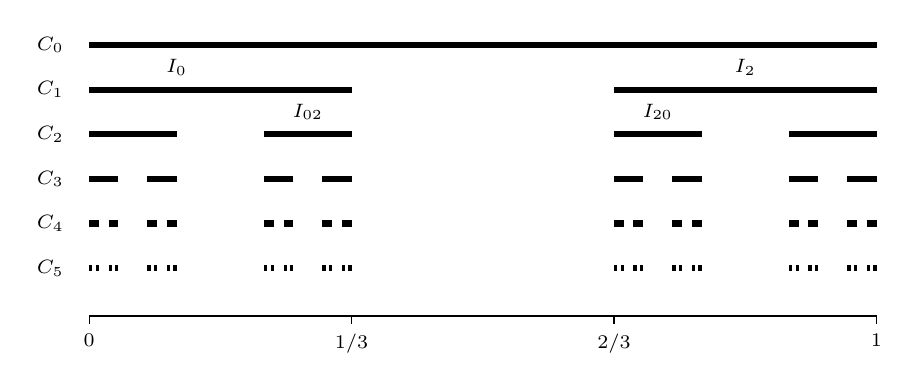
\begin{tikzpicture}[x=10cm, y=1.35cm, font=\scriptsize]
\foreach \k in {0,...,5} {\node[anchor=east] at (-0.02,-0.42*\k) {$C_{\k}$};}
\draw[line width=2.2pt] (0,0) -- (1,0);
\foreach \a in {0,0.666667} {\draw[line width=2.2pt] (\a,-0.42) -- (\a+0.333333,-0.42);}
\foreach \a in {0,0.222222,0.666667,0.888889} {\draw[line width=2.2pt] (\a,-0.84) -- (\a+0.111111,-0.84);}
\foreach \a in {0,0.074074,0.222222,0.296296,0.666667,0.740741,0.888889,0.962963} {\draw[line width=2.2pt] (\a,-1.26) -- (\a+0.037037,-1.26);}
\foreach \a in {0,0.024691,0.074074,0.098765,0.222222,0.246914,0.296296,0.320988,0.666667,0.691358,0.740741,0.765432,0.888889,0.913580,0.962963,0.987654} {\draw[line width=2.2pt] (\a,-1.68) -- (\a+0.012346,-1.68);}
\foreach \a in {0,0.008230,0.024691,0.032922,0.074074,0.082305,0.098765,0.106996,0.222222,0.230453,0.246914,0.255144,0.296296,0.304527,0.320988,0.329218,0.666667,0.674897,0.691358,0.699588,0.740741,0.748971,0.765432,0.773663,0.888889,0.897119,0.913580,0.921811,0.962963,0.971193,0.987654,0.995885} {\draw[line width=2.2pt] (\a,-2.1) -- (\a+0.004115,-2.1);}
\draw[line width=0.4pt] (0,-2.55) -- (1,-2.55);
\foreach \t/\l in {0/{$0$}, 0.333333/{$1/3$}, 0.666667/{$2/3$}, 1/{$1$}} {\draw[line width=0.4pt] (\t,-2.55) -- (\t,-2.63); \node[below] at (\t,-2.63) {\l};}
\node at (0.111111,-0.21) {$I_0$};
\node at (0.833333,-0.21) {$I_2$};
\node at (0.277778,-0.63) {$I_{02}$};
\node at (0.722222,-0.63) {$I_{20}$};
\end{tikzpicture}}{The first stages of the Cantor set. Each $C_{k+1}$ arises from $C_k$ by removing the open middle third of each of its $2^k$ intervals; the interval $I_w$ of $C_k$ consists of the points whose first $k$ ternary digits can be chosen as $w_1,\ldots,w_k\in\{0,2\}$. The Cantor set is what remains after all stages.\label{fig:cantor-set}}
\end{figure}

\begin{proposition}[Properties of the Cantor set]
\label{prop:cantor-set}
\leavevmode
\begin{enumerate}
\item A number $x\in[0,1]$ belongs to $C$ if and only if it has a base-$3$ expansion all of whose digits are $0$ or $2$. The map $\Phi\colon\{0,1\}^{\{1,2,\ldots\}}\to C$ that sends $u$ to the number with the ternary digits $2u_1,2u_2,\ldots$ is a bijection; in particular $|C|=\mathfrak c$.
\item $C$ is closed and contains no interval with more than one point.
\item Every point of $C$ is the limit of a sequence of other points of $C$.
\item $C_k$ consists of $2^k$ disjoint intervals of total length $(2/3)^k$, which tends to $0$.
\end{enumerate}
\end{proposition}

\begin{proof}
We first show that the intervals of $C_k$ are disjoint. Let $w\ne w'$ be words of length $k$ that first differ at position $j$, say $w_j=0$ and $w'_j=2$. Then
\[
s_{w'}-s_w\ge2\cdot3^{-j}-\sum_{i=j+1}^k2\cdot3^{-i}=2\cdot3^{-j}-(3^{-j}-3^{-k})=3^{-j}+3^{-k}>3^{-k},
\]
by \veqref{1}{eq:sum-geom}, so $I_{w'}$ lies to the right of $I_w$ and is separated from it by a gap of length at least $3^{-j}$.

(i) Let $x$ have a ternary expansion $(d_j)$ with digits in $\{0,2\}$. By \vcref{1}{def:expansion}, its truncations satisfy $s_k\le x\le s_k+3^{-k}$, which says that $x\in I_{(d_1,\ldots,d_k)}\subseteq C_k$, for every $k$; so $x\in C$. Conversely, let $x\in C$. For each $k$ there is exactly one word $w^{(k)}$ of length $k$ with $x\in I_{w^{(k)}}$, by the disjointness. Since $I_{w^{(k+1)}}$ lies in the interval of the word formed by its first $k$ letters, and $x$ lies in only one interval of $C_k$, the word $w^{(k+1)}$ extends $w^{(k)}$. So there is a sequence $(d_j)$ in $\{0,2\}$ with $x\in I_{(d_1,\ldots,d_k)}$ for every $k$, and this is precisely the statement that $(d_j)$ is a ternary expansion of $x$. By \vcref{1}{thm:real-expansion}\,(i), every digit sequence is the expansion of exactly one number, so $\Phi$ is well defined, and by what we have just shown it maps onto $C$. It is injective: if $u\ne u'$ first differ at position $j$, then $\Phi(u)$ and $\Phi(u')$ lie in two different, hence disjoint, intervals of $C_j$. With \cref{thm:continuum-sets}\,(ii), $|C|=\mathfrak c$.

(ii) Let $x_n\in C$ with $x_n\to x$. For each $k$, the $x_n$ lie in the $2^k$ intervals of $C_k$, so one of these intervals contains $x_n$ for infinitely many $n$; the corresponding subsequence converges to $x$, and $x$ lies in that closed interval by \vcref{1}{prop:limit-order}. So $x\in C_k$ for every $k$, and $x\in C$. By \vcref{1}{prop:closed-sequences}, $C$ is closed. Suppose that $[y,z]\subseteq C$ with $y<z$, and choose $k$ with $3^{-k}<z-y$. Both $y$ and $z$ lie in $C_k$, and they lie in different intervals of $C_k$, since each of these has length $3^{-k}<z-y$. Let $I_w=[s_w,e]$ be the interval that contains $y$, so that $y\le e<z$, and let $I_{w'}=[s_{w'},e']$ be the interval that contains $z$, so that $s_{w'}>e$. By the disjointness, the intervals of $C_k$ to the right of $I_w$ begin at least $3^{-k}$ beyond $e$, so the point $e+3^{-k}/2$ lies in no interval of $C_k$. It lies in $[y,z]$, because $e<e+3^{-k}/2<s_{w'}\le z$. This contradicts $[y,z]\subseteq C\subseteq C_k$.

(iii) Let $x\in C$ have the digits $d_j\in\{0,2\}$, and let $x_n$ be the number whose digits are those of $x$ except the $n$th, which is changed from $0$ to $2$ or from $2$ to $0$. Then $x_n\in C$, $x_n\ne x$ by the injectivity of $\Phi$, and $|x_n-x|=2\cdot3^{-n}\to0$, since by \vcref{1}{thm:real-expansion}\,(i) the numbers are the limits of their truncations, which differ by $2\cdot3^{-n}$ from the $n$th on.

(iv) $C_k$ consists of the $2^k$ disjoint intervals $I_w$ of length $3^{-k}$, and $(2/3)^k\to0$ by \veqref{1}{eq:rn-zero}.
\end{proof}

A closed set in which every point is the limit of other points of the set is called \term{perfect}; by (ii) and (iii), the Cantor set is perfect, closed, without interior points, uncountable, and contained in finite unions of intervals of arbitrarily small total length. It contains the endpoints of its intervals, such as $1/3=(0.0\overline2)_3$, and also points that are not endpoints, such as $1/4=(0.\overline{02})_3$. The Cantor set is the standard example of a set that is large in one sense and small in another, and it returns several times in this volume: Chapter~3 shows that it is compact, and Part~III shows that it has Lebesgue measure zero and builds on it the Cantor function, a continuous increasing function that is constant on every removed interval. Rudin treats it as an example in the topology of the real line~\cite{rudin1976}.

\subsection{Algebraic and Transcendental Numbers}

A real number $\alpha$ is \term{algebraic} if $P(\alpha)=0$ for some nonzero polynomial $P$ with integer coefficients, and \term{transcendental} otherwise; this is the definition of \vcref{1}{ch:numbers}, restricted to real numbers. Every rational number $p/q$ is algebraic, as a root of $qx-p$, so every transcendental number is irrational.

\begin{proposition}[Cantor]
\label{prop:algebraic-countable}
The set of real algebraic numbers is countable.
\end{proposition}

\begin{proof}
A polynomial with integer coefficients can be written as a finite word over the alphabet consisting of the ten digits, the minus sign and a separator, by listing its coefficients; distinct polynomials give distinct words. By \vcref{1}{prop:words-countable} and \vcref{1}{cor:countable}, the set of nonzero polynomials with integer coefficients is countable, and since it is not empty there is a surjection $m\mapsto P_m$ from $\mathbb N$ onto it. For an algebraic number $\alpha$, let $m(\alpha)$ be the least $m$ with $P_m(\alpha)=0$, and let $r(\alpha)$ be the number of real roots of $P_{m(\alpha)}$ that are smaller than $\alpha$; this number is finite, since a nonzero polynomial of degree $d$ has at most $d$ roots (\vcref{1}{cor:factor}). The map $\alpha\mapsto(m(\alpha),r(\alpha))$ from the algebraic numbers to $\mathbb N\times\mathbb N$ is injective: two algebraic numbers with the same $m$ are roots of the same polynomial, and if they have the same number of smaller roots, they are equal. Since $\mathbb N\times\mathbb N$ is countable, so is the set of real algebraic numbers.
\end{proof}

Since $\mathbb R$ is uncountable, transcendental numbers exist; this was Cantor's argument of 1874~\cite{cantor1874}, mentioned in Volume~I. It proves existence without exhibiting a single transcendental number. Liouville had found the first explicit examples in 1844, and published a full account in 1851, with a theorem stating that algebraic irrational numbers cannot be approximated too well by rational numbers~\cite{liouville1851,hardywright2008}.

\begin{theorem}[Liouville]
\label{thm:liouville}
Let $\alpha$ be a real root of a polynomial $P\ne0$ of degree $d\ge1$ with integer coefficients. There is a constant $c>0$ such that
\[
\Bigl|\alpha-\frac pq\Bigr|\ge\frac c{q^d}
\]
for all integers $p$ and $q$ with $q\ge1$ and $p/q\ne\alpha$.
\end{theorem}

\begin{proof}
Let $M$ be the maximum of $|P'|$ on the interval $[\alpha-1,\alpha+1]$, which exists by the extreme value theorem, \vcref{1}{thm:evt}, and put $M_1\coloneqq\max(M,1)$. The polynomial $P$ has finitely many roots; let $\rho>0$ be the smallest distance from $\alpha$ to a rational root of $P$ other than $\alpha$, or $\rho\coloneqq1$ if there is none. We show that $c\coloneqq\min(1,1/M_1,\rho)$ works. Let $p/q\ne\alpha$ with $q\ge1$. If $|\alpha-p/q|\ge1$, the inequality holds because $c\le1\le q^d$. If $P(p/q)=0$, then $p/q$ is a rational root other than $\alpha$, and $|\alpha-p/q|\ge\rho\ge c\ge c/q^d$. In the remaining case $|\alpha-p/q|<1$ and $P(p/q)\ne0$. Writing $P(x)=\sum_{i=0}^da_ix^i$, the number
\[
q^dP\Bigl(\frac pq\Bigr)=\sum_{i=0}^da_ip^iq^{d-i}
\]
is a nonzero integer, so $|P(p/q)|\ge1/q^d$. By the mean value theorem, \vcref{1}{thm:mvt}, there is $\xi$ between $\alpha$ and $p/q$, hence in $[\alpha-1,\alpha+1]$, with
\[
\frac1{q^d}\le\Bigl|P\Bigl(\frac pq\Bigr)-P(\alpha)\Bigr|=|P'(\xi)|\,\Bigl|\frac pq-\alpha\Bigr|\le M_1\Bigl|\alpha-\frac pq\Bigr| .
\]
So $|\alpha-p/q|\ge1/(M_1q^d)\ge c/q^d$.
\end{proof}

For a rational $\alpha=a/b$ the theorem with $d=1$ is elementary, $|a/b-p/q|=|aq-bp|/(bq)\ge1/(bq)$, and for $\alpha=\sqrt2$, with $d=2$, it says that $|\sqrt2-p/q|\ge c/q^2$; the Heron iterates $p/q$ come within a constant times $1/q^2$, since for $k\ge1$ their numerators and denominators satisfy $p^2-2q^2=1$, by induction from $x_1=3/2$ and $x_{k+1}=(p^2+2q^2)/(2pq)$, so that $p/q-\sqrt2=1/\bigl(q^2(p/q+\sqrt2)\bigr)$. The exponent cannot be improved for $\sqrt2$. A number that \emph{can} be approximated much better than this, for every exponent $d$, must therefore be transcendental.

\begin{corollary}[Liouville numbers]
\label{cor:liouville-numbers}
For every sequence $u=(u_k)_{k\ge1}$ with $u_k\in\{1,2\}$, the number
\[
\lambda_u\coloneqq\sum_{k=1}^\infty u_k\,10^{-k!}
\]
is transcendental, and different sequences give different numbers. Consequently, the set of transcendental numbers, and therefore also the set $\mathbb R\setminus\mathbb Q$ of irrational numbers, has the cardinality of the continuum.
\end{corollary}

\begin{proof}
The series converges by comparison with $\sum2\cdot10^{-j}$. Let $q_n\coloneqq10^{n!}$ and $p_n\coloneqq q_n\sum_{k=1}^nu_k10^{-k!}$, an integer. The exponents $k!$ with $k>n$ are distinct integers at least $(n+1)!$, so
\[
0<\lambda_u-\frac{p_n}{q_n}=\sum_{k=n+1}^\infty u_k10^{-k!}\le2\sum_{j=(n+1)!}^\infty10^{-j}=\frac{20}9\,10^{-(n+1)!}<\frac3{q_n^{n+1}} .
\]
Suppose that $\lambda_u$ were a root of a polynomial $P\ne0$ of degree $d$ with integer coefficients, and let $c$ be the constant of \cref{thm:liouville}. Since $p_n/q_n\ne\lambda_u$, the theorem gives $c/q_n^d<3/q_n^{n+1}$, that is, $c<3q_n^{d-n-1}\le3/q_n$ for $n\ge d$; as $q_n\to\infty$, this is impossible. So $\lambda_u$ is transcendental.

If $u\ne u'$ first differ at the index $m$, say $u_m=1$ and $u'_m=2$, then, since $|u'_k-u_k|\le1$ for all $k$,
\[
\lambda_{u'}-\lambda_u\ge10^{-m!}-\sum_{k=m+1}^\infty10^{-k!}\ge10^{-m!}-\frac{10}9\,10^{-(m+1)!}>0 .
\]
So $u\mapsto\lambda_u$ is an injection from $\{1,2\}^{\{1,2,\ldots\}}$, a set of cardinality $\mathfrak c$ by \cref{thm:continuum-sets}\,(ii), into the transcendental numbers. These form a subset of $\mathbb R\setminus\mathbb Q$, and \cref{thm:schroeder-bernstein-full} gives the two cardinalities.
\end{proof}

The number $\sum_k10^{-k!}=0.110001000000000000000001\ldots$, with ones in the positions $1,2,6,24,120,\ldots$, is the standard example. Liouville's numbers are artificial; the transcendence of $e$ and $\pi$, proved by Hermite in 1873 and by Lindemann in 1882 as \vcref{1}{ch:transcendental} recorded~\cite{hermite1873,lindemann1882}, requires much more delicate estimates, and so does the theorem of Gelfond and Schneider~\cite{baker1975}. Most real numbers are transcendental, in the sense of cardinality, and yet it is hard to prove that any particular number of interest is.

\section{Real Numbers in Computation: A First Look}
\label{sec:real-computation}

The construction of this chapter defines a real number by a sequence of rational approximations, and a computer works with rational approximations too. This section looks at both sides: at a real number given by a rational Cauchy sequence together with a bound for its convergence, computed in exact rational arithmetic, and at the floating-point numbers, a finite set of rational numbers that stands in for $\mathbb R$ in almost all numerical software. The computations were made on an Apple M4 Pro processor with Python~3.15, its module \code{fractions} for exact rational arithmetic, its binary64 floating-point numbers, and the array functions of the version of the stardust library of 25 November 2026; reference values were computed with the ball arithmetic of python-flint (version 0.9.0), with error bounds far below the digits shown.

\subsection{A Real Number with a Modulus}

\Cref{sec:cauchy-construction} showed that the Heron iterates satisfy $|x_m-x_n|\le\beta_k$ for all $m,n\ge k\ge1$, where
\[
\beta_k\coloneqq x_k-\frac2{x_k}=\frac{x_k^2-2}{x_k} .
\]
The bound $\beta_k$ is a rational number, computable from $x_k$ alone, without knowledge of $\sqrt2$. It answers the question that the definition of a Cauchy sequence poses, how far one must go for a given tolerance: for $\varepsilon>0$, any $k$ with $\beta_k<\varepsilon$ is an index $N$ that works. A rule that produces such an index for every tolerance is called a \term{modulus of convergence}, and a Cauchy sequence of rational numbers with a modulus is a complete description of a real number for computational purposes: to obtain the number within $\varepsilon$, compute the modulus and then one term. \Cref{tab:heron-modulus} shows the iterates in exact rational arithmetic. The bound is about twice the actual error $x_k-\sqrt2$, since $\beta_k=(x_k-\sqrt2)(x_k+\sqrt2)/x_k$, and it is squared, roughly, in every step. The smallest $k$ with $\beta_k<10^{-10}$ is $4$, with $\beta_k<10^{-100}$ it is $8$, and with $\beta_k<10^{-1000}$ it is $11$.

\begin{table}
\sdfloat{%
\begin{sdtable}{colspec={rrll}, row{1}={font=\small\bfseries}}
\toprule
$k$ & digits of $p_k$ and $q_k$ & bound $\beta_k$ & error $x_k-\sqrt2$ \\
\midrule
$1$ & $1$ & $1.67\times10^{-1}$ & $8.58\times10^{-2}$ \\
$2$ & $2$ & $4.90\times10^{-3}$ & $2.45\times10^{-3}$ \\
$3$ & $3$ & $4.25\times10^{-6}$ & $2.12\times10^{-6}$ \\
$4$ & $6$ & $3.19\times10^{-12}$ & $1.59\times10^{-12}$ \\
$5$ & $12$ & $1.80\times10^{-24}$ & $8.99\times10^{-25}$ \\
$6$ & $25$ & $5.72\times10^{-49}$ & $2.86\times10^{-49}$ \\
$7$ & $49$ & $5.78\times10^{-98}$ & $2.89\times10^{-98}$ \\
$8$ & $98$ & $5.91\times10^{-196}$ & $2.95\times10^{-196}$ \\
$11$ & $784$ & $8.01\times10^{-1568}$ & $4.00\times10^{-1568}$ \\
\bottomrule
\end{sdtable}}{Heron's iterates $x_k=p_k/q_k$ in lowest terms, from $x_0=1$, computed in exact rational arithmetic: the number of decimal digits of the numerator and of the denominator (equal in every row), the modulus bound $\beta_k=(x_k^2-2)/x_k$, which is a rational number, and the actual error, computed with $2200$ significant digits.\label{tab:heron-modulus}}
\end{table}

The price of exactness is visible in the second column: the numerator and the denominator double in length with every step, as the number of correct digits does. The iterate $x_{11}$, whose error is $4\times10^{-1568}$, is a fraction of two integers with $784$ digits each. The truncated decimal expansion of the same accuracy needs a numerator of about $1568$ digits, so the two representations are of comparable size; neither is cheap. This growth is the reason why exact rational arithmetic, mentioned in \vcref{1}{sec:rationals}, is used for proofs and for small reference computations, as in this table, but not for numerical work at scale.

\begin{note}{Computable real numbers}
Turing defined a real number to be computable if a program can produce its digits, or equivalently rational approximations within any requested tolerance~\cite{turing1936}; as \vcref{1}{sec:cardinality} observed, there are only countably many such numbers. In Bishop's constructive analysis a real number is a sequence of rational numbers $(x_n)_{n\ge1}$ with $|x_m-x_n|\le1/m+1/n$ for all $m$ and $n$, that is, a Cauchy sequence with a prescribed modulus, and two such sequences are equal if $|x_n-y_n|\le2/n$ for all $n$~\cite{bishop1967}. The definition is the construction of \cref{sec:cauchy-construction} with the moduli made explicit, and it shows what is lost when they are not: the comparison of two computable real numbers cannot in general be carried out in finitely many steps, since two sequences may agree to every precision examined so far and differ later. Weihrauch's book develops analysis on this basis~\cite{weihrauch2000}; algorithms and their cost are the subject of Volume~V.
\end{note}

\subsection{Floating-Point Numbers Are Not a Field}

A binary64 floating-point number is a rational number of the form $m\cdot2^e$ with integers $m$ and $e$ in prescribed ranges, and there are only finitely many of them: of the $2^{64}$ bit patterns, the $2^{53}$ with the largest exponent field encode infinities and NaNs, and the remaining ones represent $2^{64}-2^{53}-1=18\,437\,736\,874\,454\,810\,623$ distinct rational numbers, since $+0$ and $-0$ are equal as numbers. The decimal literal $0.1$, for instance, denotes the binary64 number
\[
\frac{3\,602\,879\,701\,896\,397}{36\,028\,797\,018\,963\,968}=\frac{3\,602\,879\,701\,896\,397}{2^{55}},
\]
which differs from $1/10$ by about $5.6\times10^{-18}$. The arithmetic operations compute the exact result and round it to a nearest floating-point number. This set with these operations is not a field, nor even a commutative ring, and \cref{tab:float-laws} shows which of the axioms of \vcref{1}{tab:axioms} and of the rules of \vcref{1}{prop:order-rules} fail.

\begin{table}
\sdfloat{%
\begin{sdtable}{colspec={lll}, row{1}={font=\small\bfseries}}
\toprule
law & expression & binary64 value \\
\midrule
A1 associativity & $(0.1+0.2)+0.3$ & $0.6000000000000001$ \\
 & $0.1+(0.2+0.3)$ & $0.6$ \\
D distributivity & $0.1\cdot(0.1+0.4)$ & $0.05$ \\
 & $0.1\cdot0.1+0.1\cdot0.4$ & $0.05000000000000001$ \\
M4 inverses & $49\cdot(1/49)$ & $0.9999999999999999$ \\
cancellation & $(10^{16}+1)-10^{16}$ & $0$ \\
$1<2\Rightarrow1+c<2+c$ & $2^{54}+1$ & $2^{54}$ \\
 & $2^{54}+2$ & $2^{54}$ \\
Archimedes & $2^{53}+1$ & $2^{53}$ \\
\bottomrule
\end{sdtable}}{Laws of an ordered field that fail in binary64 arithmetic with rounding to nearest. Each line was evaluated in Python; the decimal strings are the shortest ones that identify the binary64 results. The last line shows that adding $1$ repeatedly, starting from $0$, stops changing the value at $2^{53}$.\label{tab:float-laws}}
\end{table}

Some laws survive. Addition and multiplication are commutative, because the exact sum and product are, and rounding depends only on the exact result; $x+0=x$ and $1\cdot x=x$ hold exactly; and the order is respected in the non-strict form, $a\le b$ implies $a+c\le b+c$, because rounding to nearest is a monotone operation. What fails is everything that involves two roundings: associativity, distributivity, inverses. Each single rounding is small in relative terms, at most the unit roundoff $u=2^{-53}$ of Volume~I; indeed $1+u$ is rounded to $1$, while $1+2^{-52}$ is the next floating-point number after $1$. Their effect on a result need not be small, as the line on cancellation shows: there one rounding error of size $1$, relatively tiny compared with $10^{16}$, is the whole of the result. Floating-point arithmetic is therefore not a model of $\mathbb R$ but an approximation to it, and every statement about a computation in floating point must be accompanied by an account of the rounding errors. Developing this account, with the floating-point numbers as a finite subset of $\mathbb Q$ and rounding as a map from $\mathbb R$ onto it, is the task of Volume~VI.

\subsection{Watching an Upper Limit}

An upper limit is a statement about all sufficiently late terms, and no finite computation can determine it. What a computation can show is how the evidence accumulates. \Cref{sec:extended-limsup} proved that $\limsup\sin n=1$ and $\liminf\sin n=-1$. \Cref{tab:sin-limsup} shows the largest and the smallest value of $\sin k$ over the windows $n\le k\le10n$, located with the array functions of the library among the binary64 values of $\sin k$; the distances from $\pm1$ were then computed in ball arithmetic. The record values approach $1$ and $-1$ erratically: the window from $10^3$ to $10^4$ improves little on the one before, and the next window gains four orders of magnitude. The records are governed by rational approximations of $\pi$. The value $\sin k$ is close to $1$ when $k$ is close to $2\pi m+\pi/2$ for an integer $m$, that is, when $2k/(4m+1)$ is close to $\pi$: for $k=33$, $m=5$, the fraction is $66/21=22/7=3.142857\ldots$; for $k=51\,819$, $m=8\,247$, it is $3.14159265209\ldots$; and for $k=4\,846\,147$ it agrees with $\pi$ to thirteen digits. How close such fractions can come, and therefore how fast the records improve, depends on the continued fraction of $\pi$, in which no pattern is known.

\begin{table}
\sdfloat{%
\begin{sdtable}{colspec={rrlrl}, row{1}={font=\small\bfseries}}
\toprule
window & $k$ & $1-\sin k$ & $k$ & $1+\sin k$ \\
\midrule
$[1,10]$ & $8$ & $1.06\times10^{-2}$ & $5$ & $4.11\times10^{-2}$ \\
$[10,10^2]$ & $33$ & $8.81\times10^{-5}$ & $11$ & $9.79\times10^{-6}$ \\
$[10^2,10^3]$ & $699$ & $9.53\times10^{-6}$ & $344$ & $9.66\times10^{-6}$ \\
$[10^3,10^4]$ & $9\,929$ & $6.41\times10^{-6}$ & $9\,574$ & $6.52\times10^{-6}$ \\
$[10^4,10^5]$ & $51\,819$ & $3.03\times10^{-10}$ & $52\,174$ & $1.52\times10^{-11}$ \\
$[10^5,10^6]$ & $573\,204$ & $4.32\times10^{-14}$ & $781\,545$ & $3.06\times10^{-11}$ \\
$[10^6,10^7]$ & $4\,846\,147$ & $3.27\times10^{-14}$ & $5\,992\,555$ & $5.51\times10^{-14}$ \\
\bottomrule
\end{sdtable}}{The largest and the smallest value of $\sin k$ for integers $k$ in the window $[n,10n]$: the index $k$ of the maximum and its distance $1-\sin k$ from $1$, and the index of the minimum and its distance $1+\sin k$ from $-1$. Both distances tend to $0$ along the windows, in accordance with $\limsup\sin n=1$ and $\liminf\sin n=-1$.\label{tab:sin-limsup}}
\end{table}

The Ces\`aro means behave quite differently. Computed as cumulative sums of the binary64 sines, they were $\sigma_{10}=0.141$, $\sigma_{100}=-1.27\times10^{-3}$, $\sigma_{10^4}=1.63\times10^{-4}$, $\sigma_{10^6}=-1.17\times10^{-7}$ and $\sigma_{10^7}=1.96\times10^{-7}$, all within the bound $2.1/n$ of \cref{sec:extended-limsup}, and they agreed with the closed form of the sum there to at least eleven significant digits. The averages of a sequence can be far better behaved than the sequence, and the gap between the inequalities of \cref{cor:cesaro} is the measure of this.

\bigskip
A real number is a class of Cauchy sequences of rational numbers, and with sums, products and the order defined termwise, these classes form a complete ordered field; it contains $\mathbb Q$ as the classes of constant sequences, every representative converges to its class, and completeness holds in both forms, for Cauchy sequences and for suprema. Dedekind's cuts give the same field by a construction that uses only the order of $\mathbb Q$, at the cost of laborious algebra. Every Archimedean ordered field embeds into $\mathbb R$ in exactly one way that respects sums, products and order, and any two complete ordered fields are related by exactly one bijection that respects sums and products, so that \vcref{1}{asm:reals} describes a unique structure and is now a theorem. In an arbitrary ordered field, the existence of suprema, the convergence of bounded monotone sequences, the nested interval property with the Archimedean property, the Bolzano--Weierstrass property and the convergence of Cauchy sequences with the Archimedean property are equivalent, and so is the intermediate value property; the field of formal Laurent series shows that the Archimedean hypothesis is needed. With $\pm\infty$ added, every set of real numbers has a supremum and every sequence an upper and a lower limit, the largest and smallest limits of its subsequences, which control Ces\`aro means and the ratio and root tests and extend to functions as semicontinuity. The sets $\mathbb R^n$, $\mathbb R^{\mathbb N}$ and $C(\mathbb R)$ and the Cantor set all have the cardinality of the continuum, while the set of all functions is larger; the algebraic numbers are countable, and Liouville's theorem produces explicit transcendental numbers.

The construction of this chapter is the model for the next one. A metric space is a set with a distance, and its Cauchy sequences, its null sequences and its completion are defined exactly as here, with the distance $|p-q|$ of rational numbers replaced by a general one; the real numbers become the first example of a complete metric space, and the contraction mapping theorem, which finds solutions of equations as limits of Cauchy sequences, becomes available.

\chapternotes

The construction of the real numbers belongs to the 1870s. Méray~\cite{meray1869} and Cantor~\cite{cantor1872} defined real numbers through sequences of rational numbers that converge in the sense of Cauchy, and Heine's paper on the elements of the theory of functions, which drew on Cantor's ideas, gave a construction of the same kind~\cite{heine1872}; in the same year Dedekind published the construction by cuts~\cite{dedekind1872}. Ebbinghaus and his coauthors describe this history and both constructions~\cite{ebbinghaus1991}, and Ferreir\'os places them in the history of set theory~\cite{ferreiros2007}. Hilbert proposed in 1900 to describe the real numbers by axioms instead, among them an axiom of completeness~\cite{hilbert1900zahlbegriff}; \vcref{1}{asm:reals} is a form of this approach, and \cref{thm:reals-exist,thm:uniqueness-complete} reconcile it with the constructions. Landau's \emph{Grundlagen} builds the number systems from Peano's axioms in full detail~\cite{landau1930}, Rudin's appendix constructs the real numbers by cuts~\cite{rudin1976}, and Spivak's \emph{Calculus} ends with the construction from cuts and the proof of uniqueness~\cite{spivak2008calculus}.

The equivalence of the forms of completeness, and its failure without the Archimedean property, is the subject of Propp's article~\cite{propp2013}, which collects many further statements of calculus that are equivalent to completeness, and of Teismann's~\cite{teismann2013}; Abbott~\cite{abbott2015} and Bartle and Sherbert~\cite{bartle2011} discuss the choice of the completeness axiom at the level of a first course. Non-standard analysis is due to Robinson~\cite{robinson1966}, and the surreal numbers to Conway~\cite{conway1976}. Formal Laurent series and their order are standard algebra, and Propp names fields of this kind among his examples of ordered fields in which Cauchy sequences converge although the Archimedean property fails. Upper and lower limits, the theorems of Ces\`aro and Stolz and the comparison of the ratio and root tests are treated by Knopp~\cite{knopp1990}; special cases of \cref{thm:stolz-cesaro,thm:ratio-root}, for $b_n=n$ and for ratios with a limit, are already in Cauchy's \emph{Cours d'analyse}~\cite{cauchy1821}. Semicontinuous functions are treated by Folland~\cite{folland1999}. Kronecker's theorem, of which \cref{prop:fractional-dense} is the simplest case, is proved by Hardy and Wright~\cite{hardywright2008}, and Weyl's paper of 1916 is the classical account of uniform distribution modulo~$1$~\cite{weyl1916}.

The Schr\"oder--Bernstein theorem and the cardinalities of \cref{sec:continuum} go back to Cantor~\cite{cantor1874,cantor1878}; Halmos~\cite{halmos1960naive} and Aigner and Ziegler~\cite{aigner2018proofs} prove the theorem, and Jech~\cite{jech2003} treats the cardinal arithmetic of the continuum and the continuum hypothesis, whose independence was proved by G\"odel and Cohen~\cite{godel1940,cohen1963,cohen1964}. Liouville's theorem and his numbers appeared in 1851, after announcements in 1844~\cite{liouville1851}; Hardy and Wright prove the theorem and the transcendence of $e$ and $\pi$~\cite{hardywright2008}, and Baker's book~\cite{baker1975} gives the theory of transcendental numbers, including the theorems of Hermite~\cite{hermite1873}, Lindemann~\cite{lindemann1882}, and Gelfond and Schneider. For computable real numbers, see Turing~\cite{turing1936}, Bishop~\cite{bishop1967} and Weihrauch~\cite{weihrauch2000}; for floating-point arithmetic, Goldberg's survey~\cite{goldberg1991} and Higham's book~\cite{higham2002accuracy}, which Volume~VI follows.

\chapterreferences
